% REVIEW NOTE: The Word document's mixed manual figure/table numbering is resolved here with automatic global numbering and cross-references.
\appendix

\hypertarget{source-code-and-data-availability}{%
\chapter{Source Code and Data Availability}\label{source-code-and-data-availability}}

The complete source code underlying this thesis is openly available in the project GitHub repository:

\begin{center}
\url{https://github.com/dthemann/master_dev}
\end{center}

\noindent The repository contains the docking drivers for the three tools (AutoDock Vina, DiffDock and EquiBind), the post-hoc refinement (smina / gnina) and PoseBusters validity pipeline, the pose-comparison, transmembrane-exclusion, clustering and PandaMap interaction-fingerprint analyses for both the calibration benchmark and the Orai1 application, and the scripts that generate every figure and table reported in this document.

\hypertarget{tools-and-functions}{%
\chapter{Tools and Functions}\label{tools-and-functions}}

\hypertarget{autodock-vina-1}{%
\section{AutoDock Vina}\label{autodock-vina-1}}

AutoDock Vina is a physics-based docking tool designed to enhance speed and pose prediction accuracy in comparison to earlier AutoDock versions \cite{ref022}. AutoDock Vina combines an empirical scoring function with an efficient global optimisation strategy, sampling many candidate ligand poses in the search space and ranking them according to an analytically defined estimate of binding free energy.

The docking process in AutoDock Vina is separated in five computational steps. First, receptors and ligands are prepared removing crystallographic water molecules, adding of hydrogen atoms, assigning of atom types, calculating Gasteiger partial charges, and converting the sdf or mol2 files into PDBQT format. Defining rotatable bonds for ligands allows for the exploration of conformational flexibility in the docking process. Second, defining a three-dimensional search box allows restricting the spatial region in which the ligand may be placed. In contrast to including the entire protein surface, regions can be limited to known binding pockets for computations efficiency.

Third, Vina begins the actual sampling stage by generating random initial ligand poses within the search box, where each pose is represented through translational, rotational, and torsional degrees of freedom. These candidate poses are then refined by an iterated local search procedure in which random perturbations are followed by local optimisation, enabling the algorithm to move efficiently through the conformational landscape while avoiding complete reliance on brute-force enumeration. A central reason why this is computationally feasible is that Vina uses a smooth scoring function and precomputed interaction grids, which allow fast energy evaluation and support gradient-based local improvement using a BFGS-like quasi-Newton optimiser.

Fourth, after repeated sampling and local optimisation, Vina clusters similar poses by RMSD so that highly redundant solutions are not overrepresented in the output. Fifth, the representative poses of these clusters are ranked by predicted binding free energy, and the lowest-energy poses are returned as the most likely docking solutions. This search-and-score design makes Vina highly attractive as a baseline method because its docking behaviour is explicit, reproducible, and easy to interpret in terms of chemical interactions and search heuristics \cite{ref023}.

% The rasterised duplicate of the Vina scoring equation was omitted; the native equations below are retained.

The Vina scoring function (Equation~\ref{eq:vina-1}, \cite[p.~2]{ref022}) determines how candidate poses are ranked. In simplified form, the scoring function combines pairwise intermolecular interaction terms with a penalty for ligand flexibility, so that the total predicted affinity is the weighted sum of steric attraction, steric repulsion, hydrophobic contacts, hydrogen bonding and a torsional penalty proportional to the number of rotatable bonds. More specifically, the function includes two Gaussian steric terms, one repulsion term, one hydrophobic term, one hydrogen-bond term and one conformation-dependent penalty term \cite{ref023}.

In the formulation of Trott and Olson \cite{ref022}, the predicted binding free energy is written as a sum of distance-dependent interaction terms evaluated over every ligand--receptor atom pair. Each contribution depends not on the raw interatomic distance but on the surface distance d, the interatomic separation minus the sum of the two atoms\textquotesingle{} van der Waals radii, so that d = 0 corresponds to atoms in van der Waals contact, negative values to steric overlap, and positive values to a gap between the surfaces.

The steric contribution shared by all atom pairs is built from three of these terms, namely two attractive Gaussians and one repulsive parabola. The first Gaussian (gauss1) rewards contacts close to van der Waals distance, the second (gauss2) captures a broader, longer-range attraction centred about 3\angstrom{} beyond contact, and the repulsion term penalises interpenetration by growing quadratically once the surfaces overlap (d \textless{} 0). Combining the negative Gaussian weights with the positive repulsion weight reproduces the overall shape of a Lennard-Jones potential without its hard singularity. The remaining two terms apply only to suitable atom types, namely a piecewise-linear hydrophobic term that rewards contact between non-polar atoms, and a piecewise-linear hydrogen-bond term that rewards donor--acceptor pairs at short surface distances \cite{ref022}.

Each term enters the total with a fixed weight obtained once by non-linear regression against the measured binding affinities and native poses of a large set of protein--ligand complexes, which gives Vina its hybrid empirical and knowledge-based character \cite{ref022}. The weighted per-pair sum is separated into intermolecular and intramolecular contributions, and the reported affinity is divided by a factor that increases with the number of active rotatable bonds (1 + w \ensuremath{\cdot} N\_rot). This normalisation acts as the flexibility penalty, down-weighting highly flexible ligands that incur a larger conformational-entropy cost on binding. Because the score is evaluated analytically together with its gradient, each candidate pose can be locally minimised during the search, which is why no separate post-docking optimisation step is required \cite{ref023}.

The scoring function is defined formally as follows, using the notation and weights of Trott and Olson \cite{ref022}. The conformation-dependent score c is summed over all pairs of atoms that can move relative to one another (normally excluding atoms separated by three or fewer consecutive covalent bonds):

\begin{equation}
c\  = \ \sum_{i\  < \ j}^{}{f_{t_{i}t_{j}}\left( r_{ij} \right)}
\label{eq:vina-1}
\end{equation}

where atom i carries a type ti and f\_ti,tj is a symmetric interaction function of the interatomic distance r\_ij. The score separates into an intermolecular and an intramolecular part,

\begin{equation}
c\  = \ c_{inter}\  + \ c_{intra}
\label{eq:vina-2}
\end{equation}

and the predicted free energy of binding is read from the intermolecular part of the lowest-scoring conformation (denoted 1), while the remaining conformations are ranked with the intramolecular term of that best binding mode held fixed, so that the ranking is preserved:

\begin{equation}
s_{1}\  = \ g\left( c_{1}\  - \ c_{intra,1} \right)\  = \ g\left( c_{inter,1} \right)
\label{eq:vina-3}
\end{equation}

\begin{equation}
s_{i}\  = \ g\left( c_{i}\  - \ c_{intra,1} \right)
\label{eq:vina-4}
\end{equation}

Each interaction function is written in terms of the surface distance d\_ij, obtained from the interatomic distance by subtracting the van der Waals radii R of the two atom types (hydrogen atoms are treated implicitly, and all interactions are truncated at r\_ij = 8\angstrom{}):

\begin{equation}
f_{t_{i}t_{j}}\left( r_{ij} \right)\  \equiv \ h_{t_{i}t_{j}}\left( d_{ij} \right),\quad d_{ij}\  = \ r_{ij}\  - \ R_{t_{i}}\  - \ R_{t_{j}}
\label{eq:vina-5}
\end{equation}

The function h is a weighted sum of three steric terms common to every atom pair, plus a hydrophobic term and a hydrogen-bond term that act only on the appropriate atom types. The three steric terms are two attractive Gaussians and a repulsive parabola:

\begin{equation}
{gauss}_{1}(d)\  = \ exp\left\lbrack - \left( \frac{d}{0.5\angstrom{}} \right)^{2} \right\rbrack
\label{eq:vina-6}
\end{equation}

\begin{equation}
{gauss}_{2}(d)\  = \ exp\left\lbrack - \left( \frac{(d\  - \ 3\angstrom{})}{2\angstrom{}} \right)^{2} \right\rbrack
\label{eq:vina-7}
\end{equation}

\begin{equation}
repulsion(d)\  = \ d^{2}\quad for\quad d\  < \ 0,\quad\quad\ 0\quad for\quad d\  \geq \ 0
\label{eq:vina-8}
\end{equation}

The hydrophobic term equals 1 for d \textless{} 0.5\angstrom{} and 0 for d \textgreater{} 1.5\angstrom{}, with linear interpolation in between. The hydrogen-bond term equals 1 for d \textless{} \ensuremath{-}0.7\angstrom{} and 0 for d \textgreater{} 0, again interpolated linearly. The conformation-independent factor g then rescales the intermolecular score by the number of active rotatable bonds N\_rot between heavy atoms in the ligand:

\begin{equation}
g\left( c_{inter} \right)\  = \ \frac{c_{inter}}{\left( 1\  + \ w \cdot N_{rot} \right)}
\label{eq:vina-9}
\end{equation}

The six weights w that fix the relative contribution of each term were obtained by tuning the function against the PDBbind dataset, going beyond simple linear regression. Their values are reproduced from Table 1 of \cite{ref022} below.

\begin{longtable}[]{@{}
  >{\raggedright\arraybackslash}p{(\columnwidth - 2\tabcolsep) * \real{0.5000}}
  >{\raggedright\arraybackslash}p{(\columnwidth - 2\tabcolsep) * \real{0.5000}}@{}}
\caption{AutoDock Vina Scoring-Function Weights Reproduced from Trott and Olson}\tabularnewline
\toprule\noalign{}
{\raggedright \textbf{Weight}} & {\raggedright \textbf{Term}} \\
\midrule\noalign{}
\endfirsthead
\caption[]{AutoDock Vina Scoring-Function Weights Reproduced from Trott and Olson (continued)}\tabularnewline
\toprule\noalign{}
{\raggedright \textbf{Weight}} & {\raggedright \textbf{Term}} \\
\midrule\noalign{}
\endhead
\bottomrule\noalign{}
\endlastfoot
\ensuremath{-}0.0356 & gauss\textsubscript{1} \\
\ensuremath{-}0.00516 & gauss\textsubscript{2} \\
0.840 & repulsion \\
\ensuremath{-}0.0351 & hydrophobic \\
\ensuremath{-}0.587 & hydrogen bonding \\
0.0585 & N\_rot \\
\end{longtable}
\labelcurrenttable{tab:appendix-vina-weights}

The two Gaussian terms were introduced because they provide a smooth approximation of favourable steric complementarity between ligand and receptor atoms across relevant interatomic distances. One Gaussian term rewards close but non-overlapping contacts, while the second captures broader distance-dependent attraction, together approximating dispersive complementarity without requiring a computationally expensive all-atom physical force field. The repulsion term penalizes atomic overlap at very short distances and therefore discourages physically impossible steric clashes.

The hydrophobic term rewards favourable contacts between nonpolar atoms because burial of hydrophobic surface commonly contributes to ligand stabilization in protein pockets. The hydrogen-bond term captures favourable donor-acceptor interactions within a distance range compatible with stabilizing hydrogen bonds, which is essential because many correctly docked poses are distinguished by chemically plausible polar interactions rather than by shape alone. Finally, the torsional penalty reflects the entropic cost of binding a flexible ligand, since ligands with more rotatable bonds generally lose more conformational freedom upon binding and should therefore not be ranked as favourably as equally complementary but more rigid ligands.

The weights were chosen by Trott and Olson \cite{ref022} by empirical calibration against experimental binding affinity data, while at the same time imposing the practical requirement that the scoring function remain smooth enough for efficient local optimisation. Vina was not designed to reproduce a full physical free-energy decomposition, but rather to provide a fast and well-behaved surrogate objective that correlates reasonably with both correct pose selection and experimental affinity across a broad range of complexes. The parameter values were chosen since they offered the best compromise between speed, robustness, and predictive usefulness on benchmark datasets available to the authors at the time.

Later work built on this design philosophy and produced Vina-related variants such as smina and later Vina releases, which extended atom typing, exposed additional scoring parameters, improved local minimisation behaviour, and enabled easier rescoring or custom scoring-function development for specific benchmark settings. These later variants did not abandon the Vina paradigm but rather preserved the same central idea of a smooth empirical score combined with efficient search, making AutoDock Vina a strong and still widely used reference method in comparisons with modern AI-based docking approaches \cite{ref013}.

\hypertarget{ai-based-molecular-docking-1}{%
\section{AI-Based Molecular Docking}\label{ai-based-molecular-docking-1}}

AI-based molecular docking tools employ diverse computational strategies. Common strategies include deep-learning neural networks that predict binding poses directly from protein and ligand structures, diffusion models like DiffDock \cite{ref024} that treat docking as a generative sampling problem, geometric deep learning approaches such as EquiBind \cite{ref009}, \cite{ref010} and TankBind \cite{ref025}, \cite{ref026} that use SE(3)-equivariant networks, and regression-based models like KarmaDock \cite{ref027} and GAABind \cite{ref028} that predict binding affinities or poses with learned scoring functions. Other notable AI-based algorithms include SurfDock, DiffBindFR, DynamicBind, QuickBind, and hybrid methods like Interformer, which integrate traditional conformational searches with AI-driven scoring functions. Some methods, such as DeepDock and Uni-Mol, perform "blind docking" without requiring predefined binding sites, while others, like co-folding models, simultaneously predict structural changes in both protein and ligand to account for flexibility \cite{ref013}, \cite{ref029}.

In contrast to traditional exhaustive conformational search algorithms and empirical scoring functions, AI-based tools learn complex interaction patterns from large datasets of protein-ligand complexes to directly predict optimal binding conformations. Moreover, AI-based methods tend to be computationally efficient, which improves scalability for large-scale virtual screening.

\hypertarget{diffdock-1}{%
\subsection{DiffDock}\label{diffdock-1}}

DiffDock is a diffusion generative model (DGM). It treats protein-ligand pose prediction as a generative task rather than as the optimisation of a hand-crafted energy function. Instead of searching a scoring landscape fixed in advance by empirical interaction terms, DiffDock learns a probability distribution over correct binding poses from structural training data. It then samples candidate dockings through a reverse diffusion process \cite{ref024}.

In DiffDock, the protein and the ligand are first represented as graphs. Nodes encode chemical identity and geometry. Edges encode connectivity or spatial neighbourhood. The ligand pose is parameterized by translation, rotation, and internal torsion angles, so docking becomes a prediction over the full space of rigid-body placement and conformational flexibility. During training, a forward diffusion process gradually corrupts known experimental poses by adding noise to these variables, turning correct conformations into increasingly disordered ones.

At inference time, the reverse process runs. DiffDock starts from random noisy ligand placements and denoises them over several diffusion steps. At each step, an SE(3)-equivariant neural network predicts how to update the translation, rotation, and torsion variables so that the pose moves toward a high-probability bound conformation. Because the network is SE(3)-equivariant, its predictions transform consistently under rigid motions of the input coordinates. This equivariance is essential for reasoning over three-dimensional geometry.

A practical consequence is that DiffDock produces several plausible poses rather than one deterministic answer. This helps because real docking landscapes are often multimodal. Several poses can be chemically plausible, and near-native conformations may sit far apart in geometry. Direct regression methods struggle to capture this pattern. Finally, a separate confidence model evaluates the generated poses and ranks them by predicted reliability rather than by estimated binding free energy.

DiffDock\textquotesingle s scoring concept has two components. The first is the diffusion score model itself. It predicts the gradient of the log-probability density over poses at each noise level and thereby steers the reverse denoising trajectory toward high-likelihood regions of pose space. This is not an affinity score in the classical sense, but a learned geometric-statistical signal that tells the model how to turn a noisy pose into a more plausible one.

The second component, the confidence model, is the one directly relevant to pose ranking. Once DiffDock has generated candidate poses, the confidence network examines each predicted complex and outputs a scalar value meant to correlate with docking correctness. In particular, it reflects whether the pose falls below a conventional RMSD threshold such as 2\angstrom{} from the reference. The authors added this model because generative sampling alone does not guarantee that the top sampled pose is the best, and because practical docking needs a way to prioritize the most trustworthy candidates among many.

This ranking strategy follows from the multimodal nature of docking. Regressing a single pose can collapse several valid solutions into a physically meaningless average. Diffusion modelling was chosen because it can represent complex pose distributions, and the confidence model because it offers a calibrated way to pick the pose most likely to be near-native, even though the reverse process stays stochastic.

DiffDock's ranking behaviour is learned from large structural datasets. The effective ``parameters'' that judge poses are therefore encoded implicitly in the network weights and the training objective, not exposed as chemically interpretable constants. This lets DiffDock learn subtle interaction patterns that are hard to represent analytically, but it also makes performance depend heavily on how representative the training data are and on how well the confidence model is calibrated \cite{ref024}.

Later work extended the DiffDock framework toward flexible-pocket docking and hybrid rescoring strategies. Follow-up studies such as DiffDock-Pocket incorporated side-chain flexibility in the receptor pocket \cite{ref030}, while newer hybrid approaches pair diffusion-based pose generation with classical physics-based rescoring. This reflects a growing view. Diffusion models generate candidate poses well but can still benefit from physically motivated ranking criteria \cite{ref031}.

\hypertarget{equibind-1}{%
\subsection{EquiBind}\label{equibind-1}}

EquiBind represents a third methodological class. It is a direct geometric deep-learning approach to blind docking. Vina searches and scores many poses, and DiffDock samples and ranks many denoised ones. EquiBind instead predicts the bound pose directly, in a single forward pass of an SE(3)-equivariant neural network.

EquiBind first encodes both protein and ligand as graphs whose nodes carry chemical and geometric features. It then runs interaction-aware equivariant message passing between the two graphs. Ligand atoms gather information about the most relevant protein regions, while protein nodes encode ligand-dependent context. This matters because EquiBind uses no predefined binding site. It learns to infer both where the ligand should bind and how it should be oriented.

A central innovation is that EquiBind predicts matching sets of key points on the ligand and on the protein surface. It then computes the rigid-body transformation that best aligns the ligand key points to the protein key points, typically via a singular-value-decomposition (Kabsch-style) step. This transformation places the ligand directly into the predicted pocket. A final conformer-fitting stage adjusts internal torsions to improve local geometry while keeping the ligand chemically valid.

The full workflow therefore comprises graph construction, joint equivariant message passing, key-point prediction, rigid alignment, and torsional refinement. Compared with Vina, it drops the iterative stochastic search. Compared with DiffDock, it drops the repeated denoising steps. This runtime advantage is a main reason EquiBind is attractive for large-scale screening and for settings that need rapid blind docking.

EquiBind\textquotesingle s scoring concept departs from classical docking even more than DiffDock\textquotesingle s. In its original form, it uses no separate scoring function to rank alternative poses at inference time. Instead, it is trained with losses that directly penalize the geometric error between the predicted pose and the experimental reference. The network thus internalizes an implicit scoring rule during training and outputs a single pose that reflects that learned criterion.

The main training signals are ligand RMSD-type coordinate losses, rigid-body alignment losses, and auxiliary terms that push the predicted placement toward the correct region of the protein. These objectives were chosen for two reasons. They match the metrics used in docking evaluation, especially ligand RMSD and centroid distance, and they give stable gradients for end-to-end learning of geometric correspondences. In effect, EquiBind learns which placements are ``good'' because they minimize structural discrepancy to known complexes in the training data, not because they minimize an explicit analytic energy.

This design shapes how EquiBind should be placed in a comparative review. It is not a classical scoring-based method. It assigns no thermodynamic, affinity-like number comparable to Vina's predicted \ensuremath{\Delta}G. Nor is it a generative, uncertainty-aware sampler like DiffDock. It is a direct pose-prediction model whose ranking criteria are embedded in a learned neural representation of protein-ligand complementarity.

The authors justified this design by arguing that a sufficiently expressive SE(3)-equivariant model can learn the interaction patterns needed for docking directly from structural examples, avoiding expensive sampling and hand-crafted scoring altogether. This was one of the first influential demonstrations that blind docking can be framed as a geometric correspondence problem rather than a search over an engineered energy landscape. Later analyses, however, show that EquiBind often benefits from optional physics-based refinement when highly flexible ligands or subtle local interactions must be resolved precisely, which is why hybrid pipelines remain important in practice.

\hypertarget{optimization-tools-1}{%
\section{Optimization Tools}\label{optimization-tools-1}}

\hypertarget{smina-1}{%
\subsection{smina}\label{smina-1}}

Unlike the tools mentioned above, smina and gnina are used here as lightweight refinement tools that re-score and locally optimise generated poses. smina is a fork of AutoDock Vina developed by Koes et al. \cite{ref055}. It inherits Vina\textquotesingle s empirical scoring function and search machinery unchanged, but re-implements them so that each individual energy term can be reweighted or swapped out by the user and so that custom atom types can be defined. The energy smina optimises is therefore the Vina objective itself, an empirical, knowledge-based estimate of the binding free energy formed as a weighted sum of pairwise atom-type interaction terms, namely two attractive Gaussian steric terms, a steric-repulsion penalty, a hydrophobic contact term and a hydrogen-bond term, divided by a factor growing with the number of rotatable bonds so as to penalise ligand flexibility (the same function detailed in the Physics-Based Molecular Docking section above). Beyond full docking, smina exposes a fast local-minimisation mode that relaxes a supplied ligand pose into the nearest minimum of this energy by gradient-based optimisation, without repeating a conformational search. This makes it well suited to post-docking optimisation, since a pose seated in roughly the correct pocket but clashing sterically with the receptor can be minimised against the Vina function, removing the clash while leaving the placement essentially unchanged. Its source code is maintained on SourceForge and mirrored on GitHub \cite{ref057}.

\hypertarget{gnina-1}{%
\subsection{gnina}\label{gnina-1}}

Because gnina is in turn a fork of smina, both tools share the docking algorithm inherited from Vina \cite{ref056}, \cite{ref067}, \cite{ref068}. Conformational sampling is carried out by a set of Markov-chain Monte Carlo (MCMC) chains that repeatedly apply random perturbations, namely rigid-body translation and rotation of the whole ligand together with rotations about its rotatable bonds, to positions inside the user-defined search box. Each candidate a chain generates is driven to a local energy minimum against the Vina scoring function by gradient-based (quasi-Newton) minimisation, and a Metropolis criterion then decides whether the minimised pose is accepted as the next state of the chain. The Vina empirical energy is thus the quantity actually optimised during search and refinement in both smina and gnina. What distinguishes the two tools is how the resulting poses are finally scored and ranked.

gnina extends this lineage by replacing the hand-crafted empirical score used for ranking with a learned one \cite{ref056}, \cite{ref067}, \cite{ref068}. Once the MCMC search and Vina minimisation have produced candidate poses, gnina rescores and ranks them with an ensemble of convolutional neural networks (CNNs). Each CNN reads a three-dimensional grid of Gaussian atom-type densities, a voxelised representation of the protein-ligand complex generated by the libmolgrid library, and is trained jointly on two objectives. The first is pose scoring, a classifier, trained with a cross-entropy loss, that predicts the probability a pose lies within 2\angstrom{} RMSD of the native binding mode, reported as CNNscore. The second is binding-affinity prediction, a regression head, trained with a mean-squared-error loss that is hinged so inaccurate poses are not penalised for underestimating affinity, that predicts a binding constant on a pK (negative-log) scale, reported as CNNaffinity. Their product, CNNscore \ensuremath{\times} CNNaffinity, is exposed as CNN\_VS and is the preferred metric for ranking compounds in virtual screening \cite{ref068}. Unlike Vina\textquotesingle s \ensuremath{\Delta}G-like number, these CNN outputs are not analytic energies minimised during the search, but learned ranking criteria applied to the already-minimised poses.

The scoring CNNs come in two architectures, a linear five-convolutional-layer network (``Default2018'') and a twelve-layer densely connected network (``Dense''), and are combined into ensembles, since ensembling consistently yields better-ranked poses than any single network. gnina 1.3, the version used here, retrains these models on the updated CrossDocked2020 v1.3 dataset, ports the deep-learning backend from Caffe to PyTorch for faster CPU inference, and applies knowledge distillation to compress a five-member ensemble into a single ``fast'' student model for high-throughput screening. It also adds covalent-docking support \cite{ref067}. By default only the pose score is used to rank docked poses.

It thus occupies a hybrid position between the physics-based and AI-based approaches, namely a physics-based sampler coupled to a deep-learning scoring function, which can serve either as a standalone docking tool or, as in this work, purely as a rescoring and refinement step applied to poses produced elsewhere. It is openly available on GitHub \cite{ref058}.

The gnina CNNs are trained on the CrossDocked2020 set \cite{ref059}, millions of poses obtained by cross-docking ligands into structurally similar Protein Data Bank pockets available up to 2020 \cite{ref056}. The calibration benchmark used here is restricted to complexes released from 2021 onwards and curated so that none of the evaluated methods, e.g. DiffDock, had seen or been trained on them \cite{ref035}. The receptor-ligand pairs of the benchmark are therefore absent from gnina\textquotesingle s training data as direct entries, making the re-scoring a direct-entry temporal holdout rather than a similarity-controlled test. A later release date does not exclude homologous proteins, familiar pockets, related ligands or templates (see Section~\ref{generalisation-in-the-context-of-current-literature}).

Because both tools relax and re-score poses efficiently and use no crystal information, they provide a model-agnostic way to turn the geometrically plausible but physically strained output of the deep-learning methods into physically valid poses, i.e. a suitable tool for post-docking optimisation.

\hypertarget{docking-protocols}{%
\chapter{Docking Protocols}\label{docking-protocols}}

The three end-to-end pipelines share receptor preparation, the available RDKit ETKDG start conformer and the same downstream validity definitions, but they do not receive equal binding-site information. The benchmark is therefore a comparison of deployed workflows rather than a controlled estimate of algorithm class alone. AutoDock Vina receives a crystal-ligand-centred box, DiffDock searches the receptor blindly and EquiBind predicts or receives a pocket before local cropping. Tool-specific settings and pose budgets are summarised in Table~\ref{tab:appendix-protocols}.

All software versions were verified by invoking each binary. Docking used AutoDock Vina v1.2.7-20-g93cdc3d, a locally patched build rather than stock 1.2.7. It also used DiffDock-L (PyTorch 2.4.0 / CUDA 12.4) and a custom EquiBind pipeline (February 2025, PyTorch 2.4.1 / CUDA 12.4). Local optimisation used gnina 1.3.2 and smina (9 November 2017 build, on the Vina 1.1.2 scoring base). Receptor and ligand PDBQT preparation used Meeko 0.7.1 together with ADFRsuite-1.0 prepare\_receptor (MGLTools 1.5.7 as fallback) and Open Babel 3.1.1. Blind pocket detection for EquiBind used fpocket 4.0 and P2Rank 2.5. Physical-validity and interaction screening used PoseBusters 0.6.3 and PandaMap 4.1.0. All docking ran on a single laptop workstation with an Intel Core i9-14900HX processor (32 hardware threads) and 32 GB of system memory. AutoDock Vina ran multi-threaded on that processor at exhaustiveness 32. All GPU steps ran on a single RTX 4070 Laptop GPU (8 GB, driver 581.80, CUDA 12.4).

\hypertarget{autodock-vina-2}{%
\section{AutoDock Vina}\label{autodock-vina-2}}

AutoDock Vina \cite{ref022}, \cite{ref023} provides the classical reference. Receptors are protonated and converted to PDBQT with the stated ADFR preparation, retaining structural cofactors, while ligands use the shared start conformer. The search box is centred on the crystal ligand and extends 10 \angstrom{} beyond its bounding box on each axis. Vina runs at exhaustiveness 32, energy range 3 kcal/mol and random seed 42, retaining up to thirty ranked modes per complex. No separate post-docking optimisation is applied because Vina locally optimises poses during its native search. This crystal-centred box gives Vina more binding-site information than the blind learned pipelines and must be considered when interpreting placement and efficiency.

\hypertarget{diffdock-2}{%
\section{DiffDock}\label{diffdock-2}}

DiffDock \cite{ref024}, specifically DiffDock-L, is the diffusion-based generative method. It docks blindly over the whole receptor without a supplied search box. ESM2-650M embeddings represent the protein and the shared start conformer provides the ligand graph. Reverse diffusion uses twenty denoising steps and generates up to thirty-one candidates per complex, each ranked by native confidence. Every pose is re-scored and locally minimised with both smina and gnina. The main Results designate the smina-refined variant as DiffDock + smina, while Appendix optimisation and ranking diagnostics label raw and gnina-optimised variants explicitly.

\hypertarget{equibind-2}{%
\section{EquiBind}\label{equibind-2}}

EquiBind \cite{ref010} is a direct-regression method that natively emits one pose. To create a comparable retrospective pool, this study docks thirty fixed RDKit ETKDG conformers in unguided mode, with the receptor cropped to an 8 \angstrom{} shell around the predicted site, while fpocket- and P2Rank-guided variants are evaluated separately \cite{ref060}, \cite{ref061}. This expansion is a custom pipeline rather than native EquiBind behaviour. Every output is minimised with smina and gnina, and the main Results use the unguided EquiBind + gnina variant. Pocket-guided results test whether supplying an external site predictor improves this configured workflow, but they do not create equal information conditions with the crystal-centred Vina box.

\hypertarget{post-docking-optimisation-and-validity-screening}{%
\section{Post-Docking Optimisation and Validity Screening}\label{post-docking-optimisation-and-validity-screening}}

Because the deep-learning tools seat the ligand in approximately the right place but often in physical contact with the receptor, every DiffDock and EquiBind pose is re-scored and locally minimised with two tools in turn on the same search. The first is smina, a fork of AutoDock Vina tuned for fast local minimisation of the Vina scoring function \cite{ref055}. The second is gnina, which adds an ensemble of convolutional neural networks as a learned scoring function \cite{ref056}. Both run in local-minimisation mode within a box extended 4\angstrom{} beyond the pose, use no crystallographic information and cost only seconds per pose. This step mirrors the post-prediction energy minimisation reported alongside the PoseBusters benchmark \cite{ref035}. Its quantitative effect on physical validity and geometric accuracy is reported in the Results. All poses were finally screened with the PoseBusters validity suite, and geometric accuracy was scored as the symmetry-corrected heavy-atom RMSD to the crystal ligand.

\begin{longtable}[]{@{}
  >{\raggedright\arraybackslash}p{(\columnwidth - 6\tabcolsep) * \real{0.2433}}
  >{\raggedright\arraybackslash}p{(\columnwidth - 6\tabcolsep) * \real{0.2522}}
  >{\raggedright\arraybackslash}p{(\columnwidth - 6\tabcolsep) * \real{0.2522}}
  >{\raggedright\arraybackslash}p{(\columnwidth - 6\tabcolsep) * \real{0.2522}}@{}}
\caption{Docking-Protocol Parameters for the Three Pipelines on the Calibration Benchmark}\tabularnewline
\toprule\noalign{}
{\raggedright \textbf{Parameter}} & {\raggedright \textbf{AutoDock Vina}} & {\raggedright \textbf{DiffDock}} & {\raggedright \textbf{EquiBind}} \\
\midrule\noalign{}
\endfirsthead
\caption[]{Docking-Protocol Parameters for the Three Pipelines on the Calibration Benchmark (continued)}\tabularnewline
\toprule\noalign{}
{\raggedright \textbf{Parameter}} & {\raggedright \textbf{AutoDock Vina}} & {\raggedright \textbf{DiffDock}} & {\raggedright \textbf{EquiBind}} \\
\midrule\noalign{}
\endhead
\bottomrule\noalign{}
\endlastfoot
Method class & Physics-based (Vina) & Diffusion generative & E(3)-equivariant regression \\
Search space & Ligand box + 10\angstrom{} (0.375\angstrom{} grid) & Blind (whole receptor) & Blind; 8\angstrom{} receptor crop \\
Start conformer & RDKit ETKDG + UFF & RDKit ETKDG + UFF & 30 \ensuremath{\times} ETKDG + UFF \\
Sampling & Exhaustiveness 32; \ensuremath{\Delta}E 3 kcal/mol & 20 diffusion steps; no final noise & 30 unguided poses \\
Poses per complex & \ensuremath{\leq} 30 & \ensuremath{\leq} 30 & \ensuremath{\leq} 30 \\
Native ranking & Vina score & Model confidence & gnina affinity \\
Random seed & 42 & --- & 30 fixed seeds \\
Post-optimisation & none (native) & both refiners evaluated; primary = DiffDock + smina & both refiners evaluated; primary = EquiBind + gnina \\
Total poses (303 pairs) & 7,337 & 9,013 & \ensuremath{\approx} 9,080 \\
\end{longtable}
\labelcurrenttable{tab:appendix-protocols}

\hypertarget{posebusters-validity-checks}{%
\section{PoseBusters Validity Checks}\label{posebusters-validity-checks}}

Table~\ref{tab:appendix-posebusters-checks} lists the twenty-four individual checks of the PoseBusters validity battery referenced in the Methods (Physical and Chemical Validity). Most checks are applied to the docked pose directly, while four compare it against the co-crystallised reference ligand, and a pose is PB-valid only if it passes every one \cite{ref035}.

\begin{longtable}[]{@{}
  >{\raggedright\arraybackslash}p{(\columnwidth - 2\tabcolsep) * \real{0.3579}}
  >{\raggedright\arraybackslash}p{(\columnwidth - 2\tabcolsep) * \real{0.6421}}@{}}
\caption{PoseBusters Validity Checks}\tabularnewline
\toprule\noalign{}
{\raggedright \textbf{Check}} & {\raggedright \textbf{Description}} \\
\midrule\noalign{}
\endfirsthead
\caption[]{PoseBusters Validity Checks (continued)}\tabularnewline
\toprule\noalign{}
{\raggedright \textbf{Check}} & {\raggedright \textbf{Description}} \\
\midrule\noalign{}
\endhead
\bottomrule\noalign{}
\endlastfoot
\multicolumn{2}{@{}l@{}}{%
\textbf{Chemical validity and consistency}} \\
File loads & The docked pose can be parsed into an RDKit molecule object. \\
Sanitisation & The molecule passes RDKit's chemical sanitisation checks. \\
InChI convertible & The molecule can be converted to a standard InChI string. \\
All atoms connected & All atoms form a single connected component (no disconnected fragments). \\
No radicals & The molecule contains no unpaired electrons (radical atoms). \\
Molecular formula & The molecular formula is identical to that of the reference ligand. \\
Bonds & The bond graph (atom connectivity) is identical to the reference ligand. \\
Tetrahedral chirality & Tetrahedral stereocentres match the reference configuration. \\
Double-bond stereochemistry & Double-bond (cis/trans) configuration matches the reference. \\
\multicolumn{2}{@{}l@{}}{%
\textbf{Intramolecular validity (ligand geometry and strain)}} \\
Bond lengths & Every bond length lies within 0.75--1.25 of the RDKit distance-geometry bounds (25\% tolerance). \\
Bond angles & Every bond angle lies within 0.75--1.25 of the distance-geometry bounds. \\
Planar aromatic rings & All atoms of 5- and 6-membered aromatic rings lie within 0.25\angstrom{} of their mean plane. \\
Non-aromatic ring non-flatness & Non-aromatic 6-membered rings deviate from their mean plane by at least 0.05\angstrom{} (they are not spuriously flattened). \\
Planar double bonds & The two carbons of aliphatic C=C bonds and their four substituents lie within 0.25\angstrom{} of their mean plane. \\
Internal steric clash & Non-covalently bound atom pairs are no closer than 0.8 of the distance-geometry lower bound. \\
Internal energy ratio & The UFF energy of the pose is at most 100\ensuremath{\times} the mean energy of a 50-conformer ETKDG ensemble (no gross strain). \\
\multicolumn{2}{@{}l@{}}{%
\textbf{Intermolecular validity (ligand versus receptor)}} \\
Minimum protein--ligand distance & Protein--ligand atom pairs are farther apart than 0.75\ensuremath{\times} the sum of their van der Waals radii. \\
Minimum distance to organic cofactors & Ligand--organic-cofactor atom pairs exceed 0.75\ensuremath{\times} the sum of their van der Waals radii. \\
Minimum distance to inorganic cofactors & Ligand--inorganic-cofactor atom pairs exceed 0.75\ensuremath{\times} the sum of their covalent radii. \\
Minimum distance to waters\footnote{The two water-related checks (minimum distance to waters and volume overlap with waters) belong to the PoseBusters battery but were not evaluated in this work. Crystallographic water molecules were removed during receptor preparation, leaving no waters to test against. They are therefore reported as not applicable and treated as passing when computing PB-validity.} & Ligand--water atom pairs exceed 0.75\ensuremath{\times} the sum of their van der Waals radii. \\
Volume overlap with protein & Less than 7.5\% of the ligand volume intersects the protein (van der Waals radii scaled by 0.8). \\
Volume overlap with organic cofactors & Less than 7.5\% of the ligand volume intersects organic cofactors (radii scaled 0.8). \\
Volume overlap with inorganic cofactors & Less than 7.5\% of the ligand volume intersects inorganic cofactors (radii scaled 0.5). \\
Volume overlap with waters & Less than 7.5\% of the ligand volume intersects water molecules (radii scaled 0.5). \\
\end{longtable}
\labelcurrenttable{tab:appendix-posebusters-checks}

\hypertarget{orai1-receptor-model}{%
\chapter{Orai1 Receptor Model}\label{orai1-receptor-model}}

The docking receptor is a homology model of the human Orai1 hexamer. Each of the six identical subunits contributes residues 66 to 288 (223 residues), spanning the tail of the cytoplasmic N-terminus, the four transmembrane helices M1 to M4 and the M4 C-terminal extension, giving 1,338 residues and 10,362 heavy atoms across the assembly. The model is apo, carrying no ligand, no Ca\textsuperscript{2+} and no other heteroatoms.

The pore-lining signature residues use human Orai1 numbering. R91 is the basic cytoplasmic residue associated with the R91W severe-combined-immunodeficiency phenotype, V102 is the hydrophobic gate and E106 forms the selectivity filter \cite{ref037}. The tested ligands act at or near the pore and filter, with GSK-7975A linked to pore geometry and Synta-66 mapped to an extracellular TM1/TM3 and loop region adjacent to the filter \cite{ref070}, \cite{ref071}. They should not be described as sharing one proven intracellular binding site.

The receptor ensemble contains an equilibrated starting structure (Fr0) and three later molecular-dynamics snapshots (Fr300, Fr400 and Fr499). The files carry membrane-simulation features, including a periodic box and CHARMM-style naming. The representation follows the structural and molecular-dynamics work of the contributing Orai group \cite{ref038}, \cite{ref072}. Ensemble docking presents each ligand with several thermally sampled conformations and partly mitigates, but does not eliminate, the rigid-receptor approximation.

The four frames occupy separate molecular-dynamics coordinate systems, so raw C\ensuremath{\alpha} displacement before receptor superposition mixes conformational change with rigid-body translation and rotation and is not interpreted as structural spread. A valid cross-frame comparison should first align a stable receptor core and then report backbone RMSD. The present cross-frame pose analysis instead uses alignment-free residue-contact fingerprints folded onto residue number across the symmetric hexamer.

Pocket detection identifies the elongated ion pore as the top-ranked cavity in each frame, with M1 residues 66 to 110 and additional transmembrane residues in the more open frame. This region overlaps the functionally implicated pore and filter environment \cite{ref070}, \cite{ref071}, but it is not a conventional buried hydrophobic pocket. The complementary geometric finder returns hundreds of low-druggability cavities, illustrating why blind site selection is unusually difficult on this membrane channel.

\hypertarget{experimental-ligand-pharmacology}{%
\chapter{Experimental Ligand Pharmacology}\label{experimental-ligand-pharmacology}}

The three experimental compounds introduced with the experimental dataset in Section~\ref{experimental-dataset} are described pharmacologically here in turn, in the order GSK-7975A, Synta-66 and 2-APB (docked in its neutral form, 2abp-NH2).

GSK-7975A is a pyrazole-derived Orai blocker and the most selective of the three, though not a clean Orai1 tool in native tissue. Derler et al. report a half-maximal inhibitory concentration near 4 \ensuremath{\mu}M for both ORAI1 and ORAI3 currents, with roughly 8 \ensuremath{\mu}M against L-type voltage-gated calcium channels and above 10 \ensuremath{\mu}M against the transient receptor potential channels tested, and that micromolar figure is the value the field works from for concentration selection. Its site of action is tied to the selectivity filter, either directly or allosterically, since the pore mutant Orai1-E106D is markedly less sensitive while the outer-pore mutations D110A, D112A and D114A leave potency intact, and 2-APB-gated Orai3 is similarly resistant. The compound is active only from the extracellular side and does not disturb STIM1 puncta formation or STIM1 to Orai1 coupling, so it acts as a pore blocker rather than as an upstream inhibitor. Its block develops more slowly than that of trivalent lanthanum but far faster than BTP2, which needs hours of pre-incubation. Selectivity liabilities are real and not confined to TRPV6, which it blocks at 10 \ensuremath{\mu}M as completely and as rapidly as lanthanum. In mouse aorta its most sensitive action is on non-selective cation channel-mediated contraction, near 1.2 \ensuremath{\mu}M against roughly 12 \ensuremath{\mu}M for the voltage-gated component, so it there behaves functionally as a repolarising agent and leaves contractile store refilling essentially untouched. In a preparation with appreciable non-selective or voltage-gated conductance a GSK-7975A effect is therefore not automatically an Orai1 effect.

Synta-66 is an aryl-amide Orai1 blocker with a markedly different isoform fingerprint. It abolishes ORAI1 function while potentiating ORAI2 and leaving ORAI3 untouched, and concatemeric ORAI1-1, ORAI1-2 and ORAI1-3 dimers are inhibited whereas ORAI2-3 dimers are not, which makes it a probe of Orai1 dependence rather than a general Orai blocker. Structurally it retains an aryl amide core flanked by a fluoropyridine and a 2,3-dimethoxyaryl moiety. Waldherr et al. localise its action to an extracellular site formed by the outer parts of TM1 and TM3 together with extracellular loops 1 and 3, immediately adjacent to the selectivity filter, with docked hydrogen bonds to Asp110 and His113, reduced inhibition in the loop1 mutants L109D, H113G and Y115G and the loop3 mutants F199G, P201G and L202G, and molecular dynamics showing the compound anchoring progressively deeper towards the filter over about 100 ns. Additional sites are not excluded, but the peer-reviewed evidence points to the extracellular face rather than to both faces of the hexamer. Consistent with a filter-proximal site, E106D largely abolishes the block, STIM1 puncta formation and STIM1 to Orai1 coupling are unaffected, and the block depends on calcium-selective permeation, since in divalent-free sodium solution 10 \ensuremath{\mu}M inhibits wild-type Orai1 only partially whereas the same protocol in calcium gives complete block. Potency should therefore not be quantified under divalent-free conditions or in non-selective mutants. In glioblastoma lines the compound blocks store-operated entry almost completely at 1 and 10 \ensuremath{\mu}M in A172, LN-18 and U-87 MG without impairing viability or migration, and at 10 \ensuremath{\mu}M it modestly increased growth of LN-18 and U-87 MG, significantly for LN-18 at 48 h, while slightly increasing temozolomide sensitivity in U-87 MG.

The docking input 2abp-NH2 is native 2-APB (2-aminoethoxydiphenyl borate) in its neutral protonation state, so the pharmacology below characterises the docked molecule directly. 2-APB is the oldest and by far the least selective of the three and is better described as a bimodal modulator with two points of attack than as an inhibitor. On the channel its sign reverses with concentration, Orai1 being potentiated around 5 to 10 \ensuremath{\mu}M and blocked at 50 \ensuremath{\mu}M, Orai2 showing transient potentiation before block, and Orai3 being potentiated even at high concentration. On Orai3 it does more than gate the channel, widening the minimum pore from about 3.8 \angstrom{} to more than 5.34 \angstrom{} and destroying calcium selectivity so that monovalent ions permeate in both directions, with a smaller dilation from 3.8 to 4.6\angstrom{} measured on STIM1-activated Orai1. It also acts on the sensor. Wei et al. show that it leaves STIM1 to STIM1 interactions unchanged while enhancing the intramolecular coupling between CC1 and SOAR, locking STIM1 towards its autoinhibited resting state, an effect abolished by L258G and L416G, and that it directly inhibits the constitutively active Orai1 mutants P245T and V102A while potentiating V102C and indirectly impairs functional STIM1 to Orai1 coupling through the ETON-region residue K85. Two consequences matter for interpretation. Inhibition of puncta and inhibition of store-operated entry are dissociable, since co-expression of Orai1 abolishes the puncta effect while the entry block persists, so a 2-APB-sensitive signal identifies neither module. Application timing also changes the result, pre-incubation before store depletion inhibiting about 77\% against about 57\% for application afterwards. Its off-target breadth remains the dominant caveat, since inositol trisphosphate and ryanodine receptors, TRPC5, TRPM2 and several gap-junction subtypes are all affected, and TRPM7 block proceeds through intracellular acidification rather than direct action, a mechanism that can secondarily reach pH-sensitive conductances such as Kv1.3 in T cells and so reduce the driving force for calcium entry independently of Orai.

Read as a set, the three ligands therefore span a micromolar Orai1 and Orai3 pore block, an Orai1-selective extracellular block with an internal Orai2 contrast, and a bimodal modulator that acts both on the pore and on the STIM1 sensor. Their documented sites of action nonetheless converge on the extracellular pore mouth and the selectivity filter rather than on the conduction pathway, which is precisely what the placement criterion used in the results chapter encodes, while their differing mechanisms explain why the biologically defensible region is not identical for the three compounds. For the docking comparison this matters twice over, once because a chemically valid pose inside the transmembrane slab is implausible for any of them, and once because the size and flexibility of the three scaffolds differ enough to load the tools unevenly. Should an orthogonal chemotype be needed to cross-check an Orai1-dependence conclusion in future work, the pyrazole-core compound C79413 and the indole-like C63368, which block the CRAC current at 2.2 and 7.0 \ensuremath{\mu}M rapidly and reversibly and are unaffected by the mutations that weaken Synta-66, occupy a different region of the pore and are better characterised for that purpose than 2-APB. The docked structure represents the neutral protonation state of 2-APB. Because the aminoethyl group is partly protonated at physiological pH, poses for the cationic form are not sampled here and remain for separate validation.

\hypertarget{ranking-quality}{%
\chapter{Ranking Quality}\label{ranking-quality}}

Figures~\ref{fig:appendix-r28a} to \ref{fig:appendix-r28d} turn from whether a near-native pose exists to whether a tool can surface it. For every complex, poses are sorted by a ground-truth quality criterion and assigned an oracle rank, where rank 1 is the best pose in that tool\textquotesingle s own pool. Each panel then plots the median oracle rank at every tool-assigned rank position. Perfect ordering follows the diagonal, while random ordering centres near (N+1)/2, approximately 15.5 for thirty poses.

Because oracle rank is defined within each tool\textquotesingle s own pose pool, these panels measure ranking fidelity rather than absolute accuracy and must be read with the preceding recovery analyses. Figure~\ref{fig:appendix-r28c} is different. It reports physical-validity frequency by rank. This appendix deliberately compares native Vina ranking, raw DiffDock confidence ranking and gnina-ranked, gnina-optimised EquiBind output. These are not the same variants as the main Results, which use DiffDock + smina and EquiBind + gnina, so appendix ranking values should not replace the main headline estimates.

\begin{figure}[!htbp]
\centering
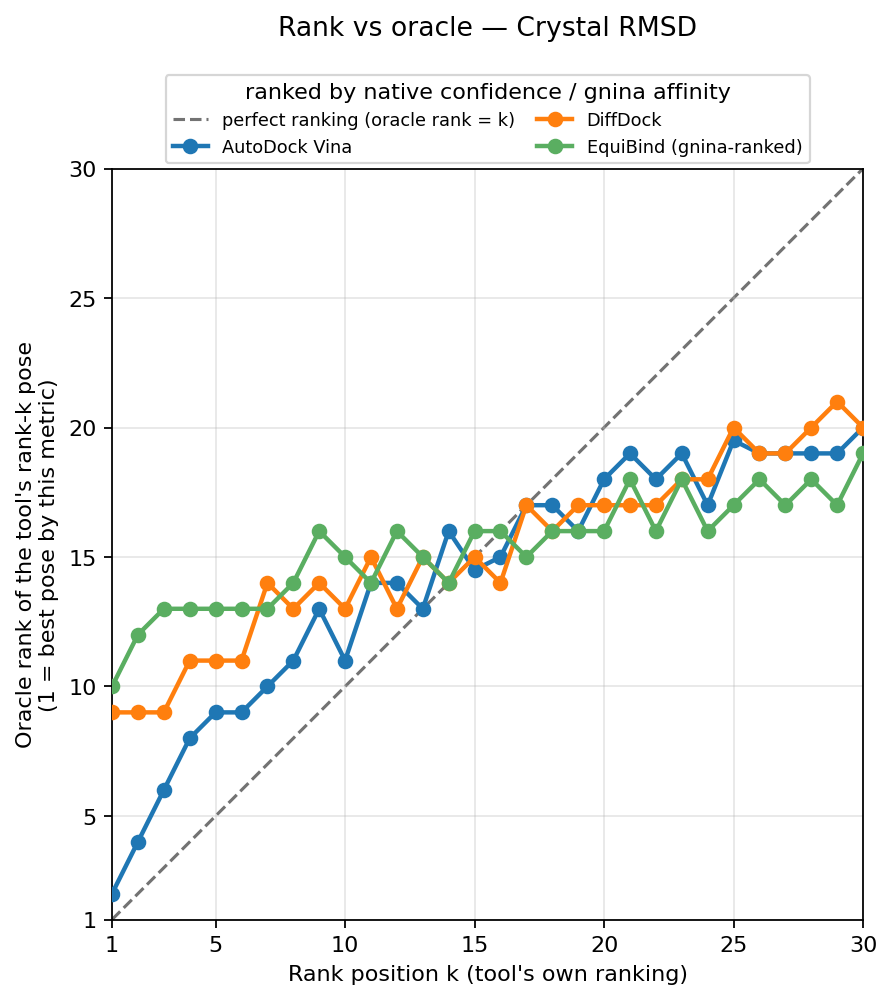
\includegraphics[width=\linewidth,height=0.78\textheight,keepaspectratio]{media/media/image29.png}
\caption{Rank versus oracle for as-placed crystal RMSD. The horizontal axis is each tool's own rank position k and the vertical axis the median oracle rank of the pose it placed at k, where oracle rank 1 is the pose closest to the crystal ligand. The dashed diagonal is perfect ranking and 15.5 is the expected oracle rank under random ordering}\label{fig:appendix-r28a}
\end{figure}

By as-placed crystal RMSD, the criterion that rewards putting the ligand in the right place, AutoDock Vina is the only tool whose ordering carries appreciable signal. Its rank-1 pose is the second best of its roughly thirty, its rank-2 pose the fourth best and its rank-3 pose the sixth best, so its curve lies closest to the diagonal at early ranks before rising towards the mid-range around k \ensuremath{\approx} 15. DiffDock and EquiBind both start far above the diagonal, with their most confident pose landing only at median oracle rank 9 and 10 respectively, so their ordering is weak, although the distance from the mid-range value shows it is not entirely absent. A tool's single most trusted pose is therefore rarely its own best-placed pose, and the ranking signal that does exist is concentrated at the top of each list.

\begin{figure}[!htbp]
\centering
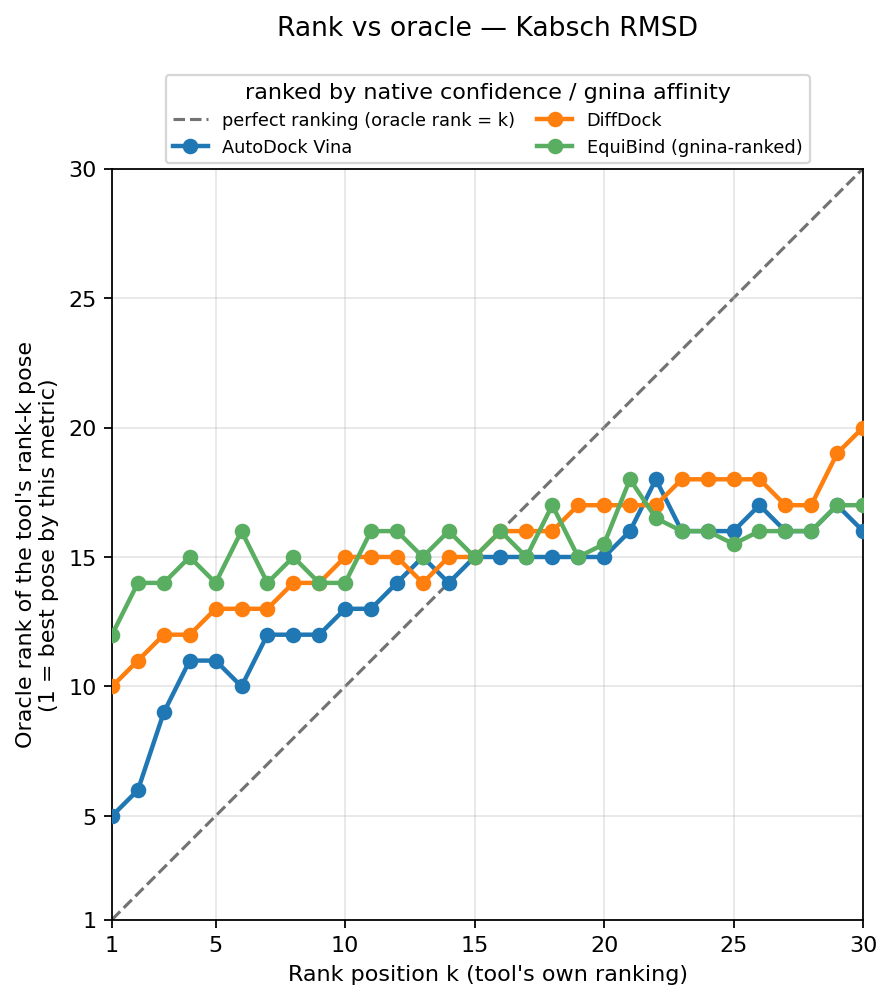
\includegraphics[width=\linewidth,height=0.78\textheight,keepaspectratio]{media/media/image30.png}
\caption{Rank versus oracle for best-fit (Kabsch) RMSD, representing internal form after optimal superposition. Axes as in Figure~\ref{fig:appendix-r28a}}\label{fig:appendix-r28b}
\end{figure}

Figure~\ref{fig:appendix-r28b} repeats the construction with best-fit Kabsch RMSD as the oracle criterion, which measures the residual conformational difference remaining after the pose is optimally superposed on the crystal ligand, that is its internal form with placement removed. Here every curve moves towards the mid-range and the advantage Vina held on placement disappears. Its rank-1 pose is now only the fifth best of its set by form, while DiffDock and EquiBind place their top pose at oracle rank 10 and 12 respectively. On form the physics-based and learned orderings are statistically indistinguishable, and DiffDock's median concordance is in fact nominally the higher of the two (\ensuremath{\tau} = 0.122 against Vina's 0.108, p = 0.504), while EquiBind's gnina order carries essentially no form signal (\ensuremath{\tau} = 0.048). No tool orders its own poses well by pure internal shape, which shows that the ranking signal Vina does possess concerns where the ligand sits rather than how its conformation is resolved.

\begin{figure}[!htbp]
\centering
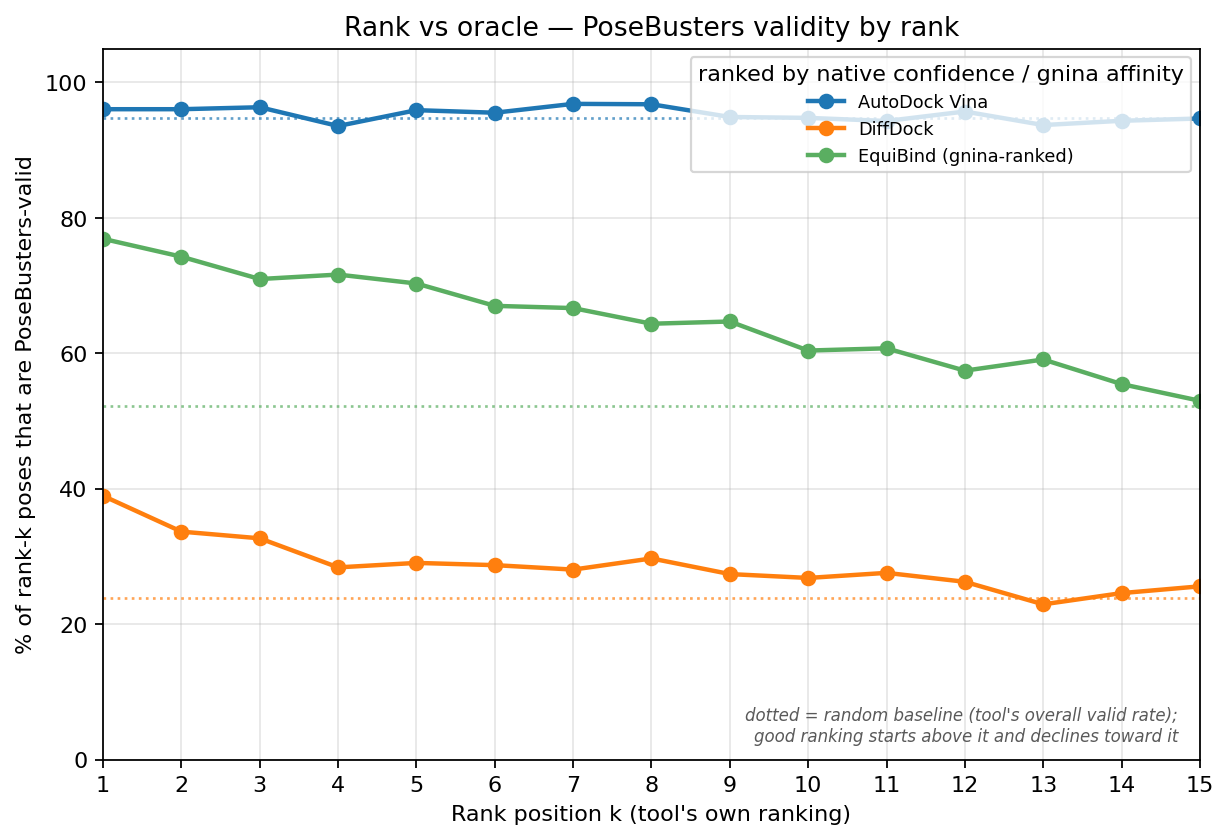
\includegraphics[width=\linewidth,height=0.78\textheight,keepaspectratio]{media/media/image31.png}
\caption{PoseBusters validity by rank. The solid curve is the percentage of rank-k poses that are PoseBusters-valid and the dotted line is each tool's overall valid rate, the random-order reference. Good ranking starts above the dotted line and declines towards it}\label{fig:appendix-r28c}
\end{figure}

Figure~\ref{fig:appendix-r28c} changes the question, because PoseBusters validity is binary and admits no oracle rank. Instead the panel plots, at each rank position, the percentage of rank-k poses that pass the PoseBusters checks, with each tool's overall valid rate drawn as a dotted random-order reference. A useful validity ranker starts above its dotted line and decays towards it as rank worsens. AutoDock Vina is essentially flat at about 94 to 97\% across all ranks, sitting on its own high baseline because nearly every Vina pose is already valid and there is little left to sort. DiffDock front-loads validity in the right direction but from a low level, falling from about 39\% at rank 1 to its 24\% baseline, so that even its most confident pose is more likely invalid than valid. The gnina-optimised, gnina-ranked EquiBind variant shows the clearest ranking signal on the plot, declining broadly, if not strictly monotonically, from about 77\% at rank 1 towards its 52\% baseline, which makes gnina affinity an effective validity sorter for these EquiBind poses even though it is a weak geometry sorter.

\begin{figure}[!htbp]
\centering
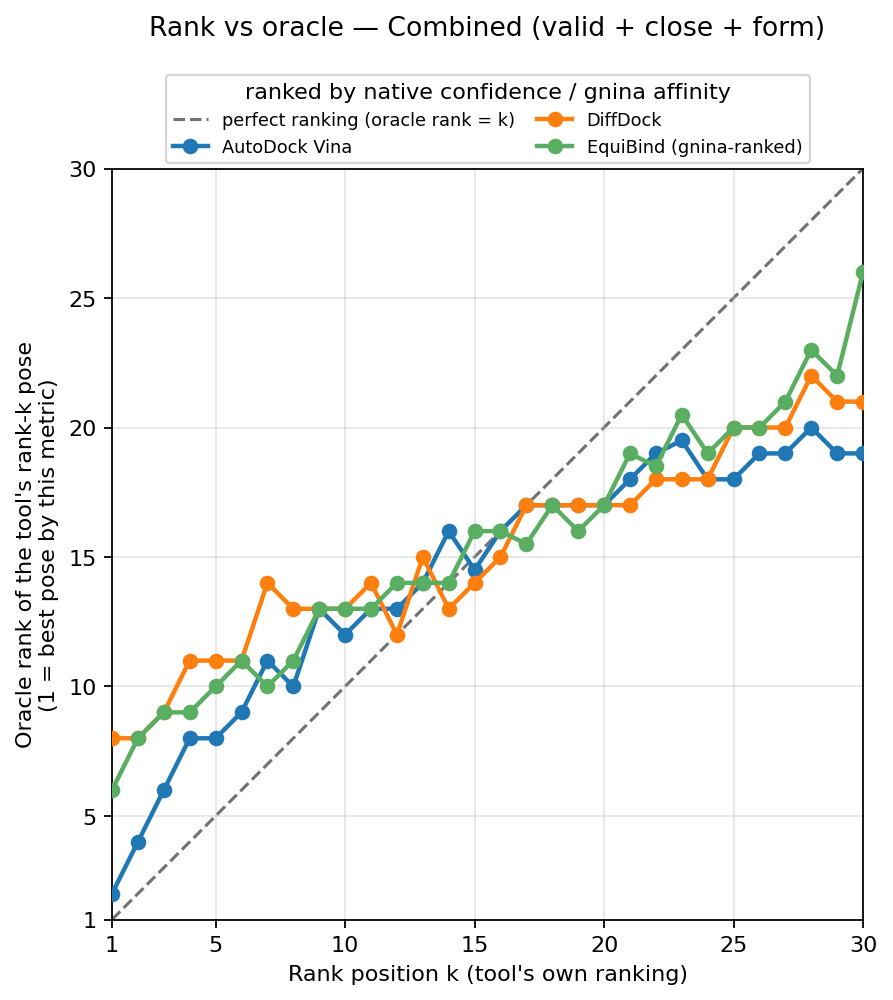
\includegraphics[width=\linewidth,height=0.78\textheight,keepaspectratio]{media/media/image32.png}
\caption{Rank versus oracle for the combined deployment criterion (validity, then placement, then form). PoseBusters-invalid poses are penalised below valid poses before valid poses are ordered by geometry. Axes as in Figure~\ref{fig:appendix-r28a}}\label{fig:appendix-r28d}
\end{figure}

Figure~\ref{fig:appendix-r28d} applies a deployment-relevant oracle criterion, in which a global penalty forces every PoseBusters-invalid pose below every valid one within a complex and the surviving valid poses are then ordered by placement and form together. It is an evaluation target rather than a selector usable in practice, since it relies on crystal RMSD, which is unavailable at real deployment time. The composite is also structurally opinionated, prioritising validity lexicographically and then summing crystal and Kabsch RMSD with equal weight, so that form is partly double-counted because as-placed RMSD already contains conformational error, and every conclusion drawn from the panel is conditional on that prespecified choice. Vina's rank-1 pose sits at oracle rank 2, almost unchanged from its crystal curve because it is already about 95\% valid and the validity-first key barely reshuffles it. DiffDock improves slightly to oracle rank 8, helped by the validity front-loading. The clearest movement is EquiBind, whose rank-1 pose rises to oracle rank 6, better than its crystal figure of 10 or Kabsch figure of 12 and now ahead of DiffDock. Because the composite rewards validity first, EquiBind's strong validity ordering lifts its whole-list concordance to a level not detectably different from Vina's, although Vina retains the better descriptive rank-1 median.

The four line charts are deliberately free of inference marks, so the formal comparison rests on three layers of distribution-free statistics computed per complex. First, a Kendall \ensuremath{\tau}-b correlation between each tool's rank order and the oracle badness order reduces every complex to a single concordance score, where +1 is perfect agreement, 0 is chance and \ensuremath{-}1 is a reversed ordering. A complex contributes only when it has at least three poses with non-constant rank and badness, which is why the validity \ensuremath{\tau} is defined solely on the mixed-validity complexes that contain both valid and invalid poses, namely 94 for Vina, 237 for DiffDock and 213 for EquiBind. The resulting per-tool medians are collected in Table~\ref{tab:appendix-ranking-concordance}.

\begin{longtable}[]{@{}
  >{\raggedright\arraybackslash}p{(\columnwidth - 6\tabcolsep) * \real{0.2500}}
  >{\raggedright\arraybackslash}p{(\columnwidth - 6\tabcolsep) * \real{0.2500}}
  >{\raggedright\arraybackslash}p{(\columnwidth - 6\tabcolsep) * \real{0.2500}}
  >{\raggedright\arraybackslash}p{(\columnwidth - 6\tabcolsep) * \real{0.2500}}@{}}
\caption{Median Per-Complex Kendall Tau-b between Tool Ranking and Oracle Badness}\tabularnewline
\toprule\noalign{}
{\raggedright Criterion} & {\raggedright AutoDock Vina} & {\raggedright DiffDock} & {\raggedright EquiBind (gnina-ranked)} \\
\midrule\noalign{}
\endfirsthead
\caption[]{Median Per-Complex Kendall Tau-b between Tool Ranking and Oracle Badness (continued)}\tabularnewline
\toprule\noalign{}
{\raggedright Criterion} & {\raggedright AutoDock Vina} & {\raggedright DiffDock} & {\raggedright EquiBind (gnina-ranked)} \\
\midrule\noalign{}
\endhead
\bottomrule\noalign{}
\endlastfoot
Crystal RMSD (placement) & 0.271 & 0.154 & 0.140 \\
Kabsch RMSD (form) & 0.108 & 0.122 & 0.048 \\
PoseBusters validity & 0.064 & 0.176 & 0.467 \\
Combined (valid + close + form) & 0.273 & 0.209 & 0.333 \\
\end{longtable}
\labelcurrenttable{tab:appendix-ranking-concordance}

A Friedman omnibus with Kendall's W as its effect size then asks whether the three tools' per-complex \ensuremath{\tau} differ, and a Wilcoxon signed-rank test with Holm correction and a matched-pairs rank-biserial effect size resolves the individual pairs. Every omnibus is highly significant (p \textless{} 0.0001), but the large sample simply confers high power, and it is Kendall's W that measures how large the systematic between-tool effect actually is. For the geometric criteria Kendall's W is only 0.050 for crystal, 0.035 for Kabsch and 0.034 for the combined score, which indicates a small between-tool effect against considerable complex-to-complex variation, so the population ordering does not translate into a reliable per-complex ranking. Only physical validity produces a substantial and stable ordering, with W = 0.341, and even that rests on just the 43 complexes that are mixed-validity for all three tools at once. On the pairwise tests Vina beats DiffDock and DiffDock beats EquiBind on crystal RMSD (rank-biserial +0.25 and +0.24, with Vina over EquiBind at +0.44), Vina and DiffDock tie on Kabsch while both beat EquiBind, EquiBind dominates both on validity (rank-biserial \ensuremath{-}0.80 against Vina and \ensuremath{-}0.89 against DiffDock), and on the combined criterion Vina beats DiffDock (p = 0.001) and EquiBind beats DiffDock (p = 0.004) while Vina and EquiBind show no significant difference (p = 0.496), which is an absence of a detected difference rather than demonstrated equivalence. One further caution applies to the tails of the curves, where the number of contributing complexes falls unequally across tools, from 303 at rank 1 to 149 for Vina, 285 for DiffDock and 302 for EquiBind at rank 30, so deep-rank comparisons rest on different subsets and are read only qualitatively. The persistence of signal into the tail is nonetheless visible, for example in EquiBind's combined median of 26 at rank 30, which shows its lowest-ranked poses being pushed towards the bottom of the pool.

Three findings follow, each requiring careful framing. AutoDock Vina is the strongest self-ranker for placement in this diagnostic, but the effect is a population tendency rather than a per-complex guarantee. Its use of the same empirical function during search and final ordering is a plausible mechanism for self-consistency \cite{ref022}, \cite{ref052}, but that mechanism is not directly tested here.

Second, both learned ranking pipelines retain a large selection gap. DiffDock\textquotesingle s native confidence and EquiBind\textquotesingle s gnina re-ranking place their top pose only around the ninth or tenth best of thirty by crystal placement, better than chance but far from the oracle. This is consistent with reported confidence-calibration and generalisation limitations for early learned docking systems \cite{ref024}, \cite{ref035}. Third, internal form is difficult for every score. All three rank Kabsch form less effectively than placement, and gnina ranking carries little form signal for EquiBind.

The single largest number in the analysis, gnina-ranked EquiBind's validity \ensuremath{\tau} of 0.467, is genuine but must not be read as evidence that EquiBind is intrinsically the better-ranking tool, because it is confounded in three ways. The validity \ensuremath{\tau} is defined only on mixed-validity complexes, and EquiBind, valid barely half the time overall, contributes 213 such information-rich complexes whereas Vina, valid about 95\% of the time, contributes only 94, and those 94 are Vina's hardest cases, so the three tools are scored on non-comparable subpopulations with only 43 in common. The ranker doing the work is gnina, a convolutional network trained to recognise realistic protein--ligand geometry, so its validity enrichment is an empirical property rather than something it was explicitly trained for, and the result largely restates that a geometry-aware model orders validity better than scores never aimed at it. And because the gnina poses are energy-minimised, gnina both optimises and ranks the EquiBind poses, so this is not a clean rescoring-only comparison nor a measurement of intrinsic EquiBind behaviour. The honest reading is that a validity-aware rescorer recovers usable ordering from a model that emits none, not that EquiBind holds an intrinsic ranking advantage, and this is single-model rescoring rather than any consensus effect.

The combined-criterion result for Vina and EquiBind is likewise structural rather than evidence of equivalence. The validity-first composite favours the gnina-ranked EquiBind subset because gnina both optimises and orders those poses, while Vina remains descriptively stronger at rank 1. The appropriate conclusion is limited to this diagnostic, namely that gnina can enrich valid EquiBind poses within mixed-validity complexes, but that does not overcome EquiBind\textquotesingle s low absolute near-native recovery or establish prospective parity with Vina.

Together, these panels illustrate the established separation between sampling and scoring \cite{ref050}, \cite{ref052}. The main recovery curves show that acceptable poses are sometimes present below rank 1, while the oracle-rank curves show that the tested scores do not reliably surface them. Vina retains the strongest placement ordering, raw learned output exhibits the physical-validity failures emphasised by PoseBusters \cite{ref035}, and gnina demonstrates that an external learned score can recover some useful ordering \cite{ref067}. Every continuous ranking result remains a population tendency, and the EquiBind validity result describes gnina\textquotesingle s behaviour on a favourable mixed-validity subset rather than an intrinsic EquiBind capability.

Tables~\ref{tab:appendix-oracle-ranks} and \ref{tab:appendix-validity-by-rank} provide the numerical data for Figure R28. Table~\ref{tab:appendix-oracle-ranks} lists median oracle rank for the crystal, Kabsch and combined criteria of Figures~\ref{fig:appendix-r28a}, \ref{fig:appendix-r28b} and \ref{fig:appendix-r28d}. Table~\ref{tab:appendix-validity-by-rank} lists PoseBusters validity by rank for Figure~\ref{fig:appendix-r28c}.

\begin{landscape}
\scriptsize
\setlength{\tabcolsep}{2pt}
\begin{longtable}[]{@{}
  >{\raggedright\arraybackslash}p{(\columnwidth - 18\tabcolsep) * \real{0.0992}}
  >{\raggedright\arraybackslash}p{(\columnwidth - 18\tabcolsep) * \real{0.0989}}
  >{\raggedright\arraybackslash}p{(\columnwidth - 18\tabcolsep) * \real{0.0999}}
  >{\raggedright\arraybackslash}p{(\columnwidth - 18\tabcolsep) * \real{0.1015}}
  >{\raggedright\arraybackslash}p{(\columnwidth - 18\tabcolsep) * \real{0.0989}}
  >{\raggedright\arraybackslash}p{(\columnwidth - 18\tabcolsep) * \real{0.0999}}
  >{\raggedright\arraybackslash}p{(\columnwidth - 18\tabcolsep) * \real{0.1015}}
  >{\raggedright\arraybackslash}p{(\columnwidth - 18\tabcolsep) * \real{0.0989}}
  >{\raggedright\arraybackslash}p{(\columnwidth - 18\tabcolsep) * \real{0.1000}}
  >{\raggedright\arraybackslash}p{(\columnwidth - 18\tabcolsep) * \real{0.1015}}@{}}
\caption{Median Oracle Rank at Positions 1--15}\tabularnewline
\toprule\noalign{}
{\raggedright \protect\hypertarget{_Toc235735959}{}{}\textbf{Rank k}} & {\raggedright \protect\hypertarget{_Toc235735960}{}{}\textbf{Vina (C)}} & {\raggedright \protect\hypertarget{_Toc235735961}{}{}\textbf{DiffDock (C)}} & {\raggedright \protect\hypertarget{_Toc235735962}{}{}\textbf{EquiBind (C)}} & {\raggedright \protect\hypertarget{_Toc235735963}{}{}\textbf{Vina (K)}} & {\raggedright \protect\hypertarget{_Toc235735964}{}{}\textbf{DiffDock (K)}} & {\raggedright \protect\hypertarget{_Toc235735965}{}{}\textbf{EquiBind (K)}} & {\raggedright \protect\hypertarget{_Toc235735966}{}{}\textbf{Vina (Cb)}} & {\raggedright \protect\hypertarget{_Toc235735967}{}{}\textbf{DiffDock (Cb)}} & {\raggedright \protect\hypertarget{_Toc235735968}{}{}\textbf{EquiBind (Cb)}} \\
\midrule\noalign{}
\endfirsthead
\caption[]{Median Oracle Rank at Positions 1--15 (continued)}\tabularnewline
\toprule\noalign{}
{\raggedright \protect\hypertarget{_Toc235735959}{}{}\textbf{Rank k}} & {\raggedright \protect\hypertarget{_Toc235735960}{}{}\textbf{Vina (C)}} & {\raggedright \protect\hypertarget{_Toc235735961}{}{}\textbf{DiffDock (C)}} & {\raggedright \protect\hypertarget{_Toc235735962}{}{}\textbf{EquiBind (C)}} & {\raggedright \protect\hypertarget{_Toc235735963}{}{}\textbf{Vina (K)}} & {\raggedright \protect\hypertarget{_Toc235735964}{}{}\textbf{DiffDock (K)}} & {\raggedright \protect\hypertarget{_Toc235735965}{}{}\textbf{EquiBind (K)}} & {\raggedright \protect\hypertarget{_Toc235735966}{}{}\textbf{Vina (Cb)}} & {\raggedright \protect\hypertarget{_Toc235735967}{}{}\textbf{DiffDock (Cb)}} & {\raggedright \protect\hypertarget{_Toc235735968}{}{}\textbf{EquiBind (Cb)}} \\
\midrule\noalign{}
\endhead
\bottomrule\noalign{}
\endlastfoot
\protect\hypertarget{_Toc235735969}{}{}1 & \protect\hypertarget{_Toc235735970}{}{}2 & \protect\hypertarget{_Toc235735971}{}{}9 & \protect\hypertarget{_Toc235735972}{}{}10 & \protect\hypertarget{_Toc235735973}{}{}5 & \protect\hypertarget{_Toc235735974}{}{}10 & \protect\hypertarget{_Toc235735975}{}{}12 & \protect\hypertarget{_Toc235735976}{}{}2 & \protect\hypertarget{_Toc235735977}{}{}8 & \protect\hypertarget{_Toc235735978}{}{}6 \\
\protect\hypertarget{_Toc235735979}{}{}2 & \protect\hypertarget{_Toc235735980}{}{}4 & \protect\hypertarget{_Toc235735981}{}{}9 & \protect\hypertarget{_Toc235735982}{}{}12 & \protect\hypertarget{_Toc235735983}{}{}6 & \protect\hypertarget{_Toc235735984}{}{}11 & \protect\hypertarget{_Toc235735985}{}{}14 & \protect\hypertarget{_Toc235735986}{}{}4 & \protect\hypertarget{_Toc235735987}{}{}8 & \protect\hypertarget{_Toc235735988}{}{}8 \\
\protect\hypertarget{_Toc235735989}{}{}3 & \protect\hypertarget{_Toc235735990}{}{}6 & \protect\hypertarget{_Toc235735991}{}{}9 & \protect\hypertarget{_Toc235735992}{}{}13 & \protect\hypertarget{_Toc235735993}{}{}9 & \protect\hypertarget{_Toc235735994}{}{}12 & \protect\hypertarget{_Toc235735995}{}{}14 & \protect\hypertarget{_Toc235735996}{}{}6 & \protect\hypertarget{_Toc235735997}{}{}9 & \protect\hypertarget{_Toc235735998}{}{}9 \\
\protect\hypertarget{_Toc235735999}{}{}4 & \protect\hypertarget{_Toc235736000}{}{}8 & \protect\hypertarget{_Toc235736001}{}{}11 & \protect\hypertarget{_Toc235736002}{}{}13 & \protect\hypertarget{_Toc235736003}{}{}11 & \protect\hypertarget{_Toc235736004}{}{}12 & \protect\hypertarget{_Toc235736005}{}{}15 & \protect\hypertarget{_Toc235736006}{}{}8 & \protect\hypertarget{_Toc235736007}{}{}11 & \protect\hypertarget{_Toc235736008}{}{}9 \\
\protect\hypertarget{_Toc235736009}{}{}5 & \protect\hypertarget{_Toc235736010}{}{}9 & \protect\hypertarget{_Toc235736011}{}{}11 & \protect\hypertarget{_Toc235736012}{}{}13 & \protect\hypertarget{_Toc235736013}{}{}11 & \protect\hypertarget{_Toc235736014}{}{}13 & \protect\hypertarget{_Toc235736015}{}{}14 & \protect\hypertarget{_Toc235736016}{}{}8 & \protect\hypertarget{_Toc235736017}{}{}11 & \protect\hypertarget{_Toc235736018}{}{}10 \\
\protect\hypertarget{_Toc235736019}{}{}6 & \protect\hypertarget{_Toc235736020}{}{}9 & \protect\hypertarget{_Toc235736021}{}{}11 & \protect\hypertarget{_Toc235736022}{}{}13 & \protect\hypertarget{_Toc235736023}{}{}10 & \protect\hypertarget{_Toc235736024}{}{}13 & \protect\hypertarget{_Toc235736025}{}{}16 & \protect\hypertarget{_Toc235736026}{}{}9 & \protect\hypertarget{_Toc235736027}{}{}11 & \protect\hypertarget{_Toc235736028}{}{}11 \\
\protect\hypertarget{_Toc235736029}{}{}7 & \protect\hypertarget{_Toc235736030}{}{}10 & \protect\hypertarget{_Toc235736031}{}{}14 & \protect\hypertarget{_Toc235736032}{}{}13 & \protect\hypertarget{_Toc235736033}{}{}12 & \protect\hypertarget{_Toc235736034}{}{}13 & \protect\hypertarget{_Toc235736035}{}{}14 & \protect\hypertarget{_Toc235736036}{}{}11 & \protect\hypertarget{_Toc235736037}{}{}14 & \protect\hypertarget{_Toc235736038}{}{}10 \\
\protect\hypertarget{_Toc235736039}{}{}8 & \protect\hypertarget{_Toc235736040}{}{}11 & \protect\hypertarget{_Toc235736041}{}{}13 & \protect\hypertarget{_Toc235736042}{}{}14 & \protect\hypertarget{_Toc235736043}{}{}12 & \protect\hypertarget{_Toc235736044}{}{}14 & \protect\hypertarget{_Toc235736045}{}{}15 & \protect\hypertarget{_Toc235736046}{}{}10 & \protect\hypertarget{_Toc235736047}{}{}13 & \protect\hypertarget{_Toc235736048}{}{}11 \\
\protect\hypertarget{_Toc235736049}{}{}9 & \protect\hypertarget{_Toc235736050}{}{}13 & \protect\hypertarget{_Toc235736051}{}{}14 & \protect\hypertarget{_Toc235736052}{}{}16 & \protect\hypertarget{_Toc235736053}{}{}12 & \protect\hypertarget{_Toc235736054}{}{}14 & \protect\hypertarget{_Toc235736055}{}{}14 & \protect\hypertarget{_Toc235736056}{}{}13 & \protect\hypertarget{_Toc235736057}{}{}13 & \protect\hypertarget{_Toc235736058}{}{}13 \\
\protect\hypertarget{_Toc235736059}{}{}10 & \protect\hypertarget{_Toc235736060}{}{}11 & \protect\hypertarget{_Toc235736061}{}{}13 & \protect\hypertarget{_Toc235736062}{}{}15 & \protect\hypertarget{_Toc235736063}{}{}13 & \protect\hypertarget{_Toc235736064}{}{}15 & \protect\hypertarget{_Toc235736065}{}{}14 & \protect\hypertarget{_Toc235736066}{}{}12 & \protect\hypertarget{_Toc235736067}{}{}13 & \protect\hypertarget{_Toc235736068}{}{}13 \\
\protect\hypertarget{_Toc235736069}{}{}11 & \protect\hypertarget{_Toc235736070}{}{}14 & \protect\hypertarget{_Toc235736071}{}{}15 & \protect\hypertarget{_Toc235736072}{}{}14 & \protect\hypertarget{_Toc235736073}{}{}13 & \protect\hypertarget{_Toc235736074}{}{}15 & \protect\hypertarget{_Toc235736075}{}{}16 & \protect\hypertarget{_Toc235736076}{}{}13 & \protect\hypertarget{_Toc235736077}{}{}14 & \protect\hypertarget{_Toc235736078}{}{}13 \\
\protect\hypertarget{_Toc235736079}{}{}12 & \protect\hypertarget{_Toc235736080}{}{}14 & \protect\hypertarget{_Toc235736081}{}{}13 & \protect\hypertarget{_Toc235736082}{}{}16 & \protect\hypertarget{_Toc235736083}{}{}14 & \protect\hypertarget{_Toc235736084}{}{}15 & \protect\hypertarget{_Toc235736085}{}{}16 & \protect\hypertarget{_Toc235736086}{}{}13 & \protect\hypertarget{_Toc235736087}{}{}12 & \protect\hypertarget{_Toc235736088}{}{}14 \\
\protect\hypertarget{_Toc235736089}{}{}13 & \protect\hypertarget{_Toc235736090}{}{}13 & \protect\hypertarget{_Toc235736091}{}{}15 & \protect\hypertarget{_Toc235736092}{}{}15 & \protect\hypertarget{_Toc235736093}{}{}15 & \protect\hypertarget{_Toc235736094}{}{}14 & \protect\hypertarget{_Toc235736095}{}{}15 & \protect\hypertarget{_Toc235736096}{}{}14 & \protect\hypertarget{_Toc235736097}{}{}15 & \protect\hypertarget{_Toc235736098}{}{}14 \\
\protect\hypertarget{_Toc235736099}{}{}14 & \protect\hypertarget{_Toc235736100}{}{}16 & \protect\hypertarget{_Toc235736101}{}{}14 & \protect\hypertarget{_Toc235736102}{}{}14 & \protect\hypertarget{_Toc235736103}{}{}14 & \protect\hypertarget{_Toc235736104}{}{}15 & \protect\hypertarget{_Toc235736105}{}{}16 & \protect\hypertarget{_Toc235736106}{}{}16 & \protect\hypertarget{_Toc235736107}{}{}13 & \protect\hypertarget{_Toc235736108}{}{}14 \\
\protect\hypertarget{_Toc235736109}{}{}15 & \protect\hypertarget{_Toc235736110}{}{}14 & \protect\hypertarget{_Toc235736111}{}{}15 & \protect\hypertarget{_Toc235736112}{}{}16 & \protect\hypertarget{_Toc235736113}{}{}15 & \protect\hypertarget{_Toc235736114}{}{}15 & \protect\hypertarget{_Toc235736115}{}{}15 & \protect\hypertarget{_Toc235736116}{}{}14 & \protect\hypertarget{_Toc235736117}{}{}14 & \protect\hypertarget{_Toc235736118}{}{}16 \\
\end{longtable}
\labelcurrenttable{tab:appendix-oracle-ranks}
\end{landscape}

\begin{landscape}
\scriptsize
\setlength{\tabcolsep}{2pt}
\begin{longtable}[]{@{}
  >{\raggedright\arraybackslash}p{(\columnwidth - 6\tabcolsep) * \real{0.2500}}
  >{\raggedright\arraybackslash}p{(\columnwidth - 6\tabcolsep) * \real{0.2500}}
  >{\raggedright\arraybackslash}p{(\columnwidth - 6\tabcolsep) * \real{0.2500}}
  >{\raggedright\arraybackslash}p{(\columnwidth - 6\tabcolsep) * \real{0.2500}}@{}}
\caption{PoseBusters Validity by Rank}\tabularnewline
\toprule\noalign{}
{\raggedright \protect\hypertarget{_Toc235736119}{}{}\textbf{Rank k}} & {\raggedright \protect\hypertarget{_Toc235736120}{}{}\textbf{AutoDock Vina}} & {\raggedright \protect\hypertarget{_Toc235736121}{}{}\textbf{DiffDock}} & {\raggedright \protect\hypertarget{_Toc235736122}{}{}\textbf{EquiBind (gnina-ranked)}} \\
\midrule\noalign{}
\endfirsthead
\caption[]{PoseBusters Validity by Rank (continued)}\tabularnewline
\toprule\noalign{}
{\raggedright \protect\hypertarget{_Toc235736119}{}{}\textbf{Rank k}} & {\raggedright \protect\hypertarget{_Toc235736120}{}{}\textbf{AutoDock Vina}} & {\raggedright \protect\hypertarget{_Toc235736121}{}{}\textbf{DiffDock}} & {\raggedright \protect\hypertarget{_Toc235736122}{}{}\textbf{EquiBind (gnina-ranked)}} \\
\midrule\noalign{}
\endhead
\bottomrule\noalign{}
\endlastfoot
\protect\hypertarget{_Toc235736123}{}{}1 & \protect\hypertarget{_Toc235736124}{}{}96 & \protect\hypertarget{_Toc235736125}{}{}39 & \protect\hypertarget{_Toc235736126}{}{}77 \\
\protect\hypertarget{_Toc235736127}{}{}2 & \protect\hypertarget{_Toc235736128}{}{}96 & \protect\hypertarget{_Toc235736129}{}{}34 & \protect\hypertarget{_Toc235736130}{}{}74 \\
\protect\hypertarget{_Toc235736131}{}{}3 & \protect\hypertarget{_Toc235736132}{}{}96 & \protect\hypertarget{_Toc235736133}{}{}33 & \protect\hypertarget{_Toc235736134}{}{}71 \\
\protect\hypertarget{_Toc235736135}{}{}4 & \protect\hypertarget{_Toc235736136}{}{}94 & \protect\hypertarget{_Toc235736137}{}{}28 & \protect\hypertarget{_Toc235736138}{}{}72 \\
\protect\hypertarget{_Toc235736139}{}{}5 & \protect\hypertarget{_Toc235736140}{}{}96 & \protect\hypertarget{_Toc235736141}{}{}29 & \protect\hypertarget{_Toc235736142}{}{}70 \\
\protect\hypertarget{_Toc235736143}{}{}6 & \protect\hypertarget{_Toc235736144}{}{}96 & \protect\hypertarget{_Toc235736145}{}{}29 & \protect\hypertarget{_Toc235736146}{}{}67 \\
\protect\hypertarget{_Toc235736147}{}{}7 & \protect\hypertarget{_Toc235736148}{}{}97 & \protect\hypertarget{_Toc235736149}{}{}28 & \protect\hypertarget{_Toc235736150}{}{}67 \\
\protect\hypertarget{_Toc235736151}{}{}8 & \protect\hypertarget{_Toc235736152}{}{}97 & \protect\hypertarget{_Toc235736153}{}{}30 & \protect\hypertarget{_Toc235736154}{}{}64 \\
\protect\hypertarget{_Toc235736155}{}{}9 & \protect\hypertarget{_Toc235736156}{}{}95 & \protect\hypertarget{_Toc235736157}{}{}27 & \protect\hypertarget{_Toc235736158}{}{}65 \\
\protect\hypertarget{_Toc235736159}{}{}10 & \protect\hypertarget{_Toc235736160}{}{}95 & \protect\hypertarget{_Toc235736161}{}{}27 & \protect\hypertarget{_Toc235736162}{}{}60 \\
\protect\hypertarget{_Toc235736163}{}{}11 & \protect\hypertarget{_Toc235736164}{}{}94 & \protect\hypertarget{_Toc235736165}{}{}28 & \protect\hypertarget{_Toc235736166}{}{}61 \\
\protect\hypertarget{_Toc235736167}{}{}12 & \protect\hypertarget{_Toc235736168}{}{}96 & \protect\hypertarget{_Toc235736169}{}{}26 & \protect\hypertarget{_Toc235736170}{}{}57 \\
\protect\hypertarget{_Toc235736171}{}{}13 & \protect\hypertarget{_Toc235736172}{}{}94 & \protect\hypertarget{_Toc235736173}{}{}23 & \protect\hypertarget{_Toc235736174}{}{}59 \\
\protect\hypertarget{_Toc235736175}{}{}14 & \protect\hypertarget{_Toc235736176}{}{}94 & \protect\hypertarget{_Toc235736177}{}{}25 & \protect\hypertarget{_Toc235736178}{}{}55 \\
\protect\hypertarget{_Toc235736179}{}{}15 & \protect\hypertarget{_Toc235736180}{}{}95 & \protect\hypertarget{_Toc235736181}{}{}26 & \protect\hypertarget{_Toc235736182}{}{}53 \\
\end{longtable}
\labelcurrenttable{tab:appendix-validity-by-rank}
\end{landscape}

\hypertarget{dataset}{%
\chapter{Dataset}\label{dataset}}

The PoseBusters benchmark provides 308 high-resolution protein-ligand crystal structures released after 2021 for testing generated poses \cite{ref035}. The release window reduces exact-entry overlap with the nominal training cutoff of early learned docking models, but it does not exclude related proteins, ligands, pockets or templates. The present study maps the chemical and structural breadth of the source set and compares it with the three Orai1-related docking inputs.

\hypertarget{composition-and-provenance}{%
\section{Composition and Provenance}\label{composition-and-provenance}}

Each of the 308 entries pairs one receptor with one cognate ligand, every complex carrying a distinct PDB identifier and a distinct ligand (308 unique PDB IDs and 308 unique chemical-component codes)\footnote{For every entry the benchmark provides four files, namely the receptor stripped of solvent but retaining its cofactors (*\_protein.pdb), all crystallographic instances of the ligand of interest (*\_ligands.sdf), the single chosen crystal instance that serves as the ground-truth answer pose (*\_ligand.sdf), and one computer-generated starting conformer produced with RDKit's ETKDGv3 algorithm followed by UFF minimisation (*\_ligand\_start\_conf.sdf).}. The crystallographic pose is the experimentally validated reference for scoring every docked pose, while the generated start conformer mimics the ligand information a docking engine sees at run time.

The experimentally resolved ligand conformations provide a reference for symmetry-corrected pose comparison. However, a later PDB release date is not proof that the biological or chemical pattern was absent from training data. Homology-, pocket-, scaffold- and template-similarity analyses are needed before making a strong no-leakage claim. Multiple crystallographic copies of the same ligand within a structure are handled by the stated symmetry-corrected comparison.

\hypertarget{ligand-physicochemical-profile}{%
\section{Ligand Physicochemical Profile}\label{ligand-physicochemical-profile}}

The 308 source ligands cover a wide region of chemical space. The median ligand has 24 heavy atoms, with an interquartile range of 16 to 32 and a full range of 6 to 64, and a median molecular weight of 359 Da. The distributions are right-skewed and extend beyond 600 Da, reflecting peptides, nucleotides, sugars and cofactor-like molecules alongside conventional small molecules (Figure~\ref{fig:appendix-dataset-1}). The median ligand has five rotatable bonds, six hydrogen-bond acceptors, three donors and a topological polar surface area of 107 \angstrom{}\textsuperscript{2}.

\begin{figure}[!htbp]
\centering

\includegraphics[width=\linewidth,height=0.78\textheight,keepaspectratio]{media/media/image33.png}
\caption{Univariate distributions of twelve physicochemical attributes across the 308 benchmark ligands}\label{fig:appendix-dataset-1}
\end{figure}

\begin{longtable}[]{@{}
  >{\raggedright\arraybackslash}p{(\columnwidth - 6\tabcolsep) * \real{0.3528}}
  >{\raggedright\arraybackslash}p{(\columnwidth - 6\tabcolsep) * \real{0.1472}}
  >{\raggedright\arraybackslash}p{(\columnwidth - 6\tabcolsep) * \real{0.2500}}
  >{\raggedright\arraybackslash}p{(\columnwidth - 6\tabcolsep) * \real{0.2500}}@{}}
\caption{Distribution of Principal Ligand Descriptors in the PoseBusters Subset}\tabularnewline
\toprule\noalign{}
{\raggedright \textbf{Descriptor}} & {\raggedright \textbf{Median}} & {\raggedright \textbf{IQR (25--75\,\%)}} & {\raggedright \textbf{Range (min--max)}} \\
\midrule\noalign{}
\endfirsthead
\caption[]{Distribution of Principal Ligand Descriptors in the PoseBusters Subset (continued)}\tabularnewline
\toprule\noalign{}
{\raggedright \textbf{Descriptor}} & {\raggedright \textbf{Median}} & {\raggedright \textbf{IQR (25--75\,\%)}} & {\raggedright \textbf{Range (min--max)}} \\
\midrule\noalign{}
\endhead
\bottomrule\noalign{}
\endlastfoot
Heavy atoms & 24 & 16--32 & 6--64 \\
Molecular weight (Da) & 359 & 236--462 & 100--872 \\
Rotatable bonds & 5 & 2--7 & 0--20 \\
H-bond acceptors & 6 & 3--9 & 0--21 \\
H-bond donors & 3 & 2--5 & 0--13 \\
TPSA (\angstrom{}\textsuperscript{2}) & 107 & 66--160 & 0--384 \\
cLogP & 0.9 & \ensuremath{-}1.6--3.2 & \ensuremath{-}8.4--14.0 \\
Fraction sp\textsuperscript{3} C & 0.41 & 0.23--0.57 & 0.00--1.00 \\
QED & 0.44 & 0.29--0.60 & 0.04--0.91 \\
Ring count & 3 & 1--4 & 0--8 \\
\end{longtable}
\labelcurrenttable{tab:appendix-ligand-distribution}

\hypertarget{drug-likeness}{%
\section{Drug-Likeness}\label{drug-likeness}}

Drug-likeness metrics confirm that the set deliberately reaches past classical small-molecule drug space. Under Lipinski's rule of five,\footnote{Lipinski's ``rule of five'' is a heuristic for oral drug-likeness. Poor absorption or permeation is more likely when a compound has more than five hydrogen-bond donors, more than ten hydrogen-bond acceptors, a molecular weight above 500 Da, or a calculated logP (cLogP) above 5, each threshold being a multiple of five. See C. A. Lipinski, F. Lombardo, B. W. Dominy and P. J. Feeney, ``Experimental and computational approaches to estimate solubility and permeability in drug discovery and development settings'', Advanced Drug Delivery Reviews, 1997, 23 (1--3), 3--25 (DOI: 10.1016/S0169-409X(96)00423-1).} 83\% of ligands incur at most one violation and 65\% none at all, yet a substantial 17\% violate two or more criteria (Figure~\ref{fig:appendix-dataset-2}). The quantitative estimate of drug-likeness (QED) sits at a median of just 0.44, and only 67\% of ligands clear the 0.34 threshold usually called ``attractive''. This spread is intentional. Keeping polar, charged and oversized ligands stresses each method's ability to generalise rather than rewarding performance on an easy, lead-like subset.

\begin{figure}[!htbp]
\centering

\includegraphics[width=\linewidth,height=0.78\textheight,keepaspectratio]{media/media/image34.png}
\caption{Drug-likeness of the benchmark ligands. Lipinski rule-of-five violation counts (left), overall rule-of-five compliance (centre) and the QED distribution (right)}\label{fig:appendix-dataset-2}
\end{figure}

\hypertarget{elemental-and-charge-composition}{%
\section{Elemental and Charge Composition}\label{elemental-and-charge-composition}}

The elemental make-up widens the challenge further (Figure~\ref{fig:appendix-dataset-3}). Roughly a quarter of the ligands contain phosphorus (25\%) or sulfur (24\%), 22\% carry at least one halogen, and metal atoms are essentially absent from the ligand records. Net formal charges are uncommon, since only 3\% of ligands are charged and the vast majority are neutral, but the heteroatom count is high and broadly spread (median 8, reaching nearly 30), matching the many nucleotide- and phosphate-containing species. These are exactly the features that the physical and chemical validity checks, namely protonation, geometry and steric clashes, probe most sharply.

\begin{figure}[!htbp]
\centering
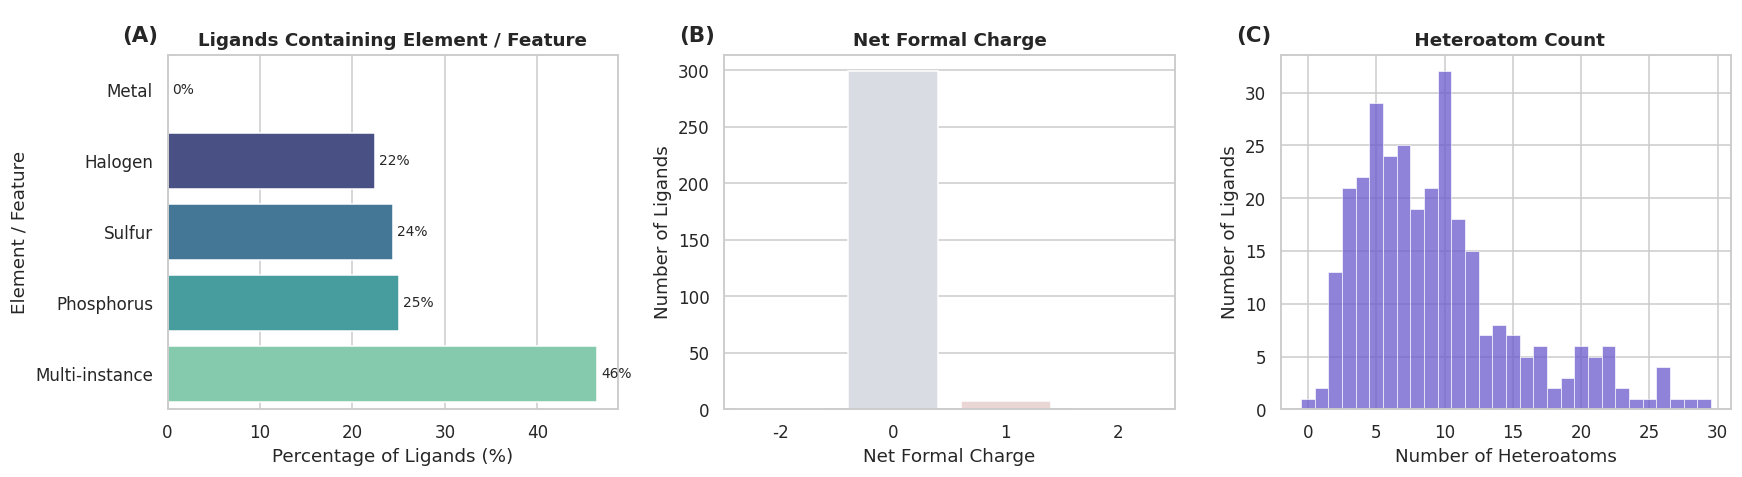
\includegraphics[width=\linewidth,height=0.78\textheight,keepaspectratio]{media/media/image35.png}
\caption{Elemental and charge composition. Prevalence of selected elements and features (left), formal-charge distribution (centre) and heteroatom counts (right)}\label{fig:appendix-dataset-3}
\end{figure}

\hypertarget{joint-distributions-and-correlation-structure}{%
\section{Joint Distributions and Correlation Structure}\label{joint-distributions-and-correlation-structure}}

The descriptors are considerably interdependent (Figure~\ref{fig:appendix-dataset-4}). The size-related quantities, namely heavy-atom count, molecular weight, hydrogen-bond acceptor count, polar surface area and heteroatom count, correlate strongly and positively, while QED falls as molecules grow larger and more polar. Lipophilicity runs opposite to polar surface area, and the sp\textsuperscript{3}-carbon fraction opposes aromatic-ring count, separating flat aromatic scaffolds from saturated three-dimensional ones. The two-dimensional mappings make this explicit. Heavy-atom and rotatable-bond counts rise together (r = +0.70) (Figure~\ref{fig:appendix-dataset-5}\,(A)), mass and polar surface area co-vary (r = +0.46), lipophilicity and polarity trade off (r = \ensuremath{-}0.61), and drug-likeness declines with size (r = \ensuremath{-}0.52) (Figure~\ref{fig:appendix-dataset-5}). The pairwise joint distributions of the six core descriptors (Figure~\ref{fig:appendix-dataset-6}) confirm that the benchmark forms one broad cloud rather than distinct clusters.

\begin{figure}[!htbp]
\centering
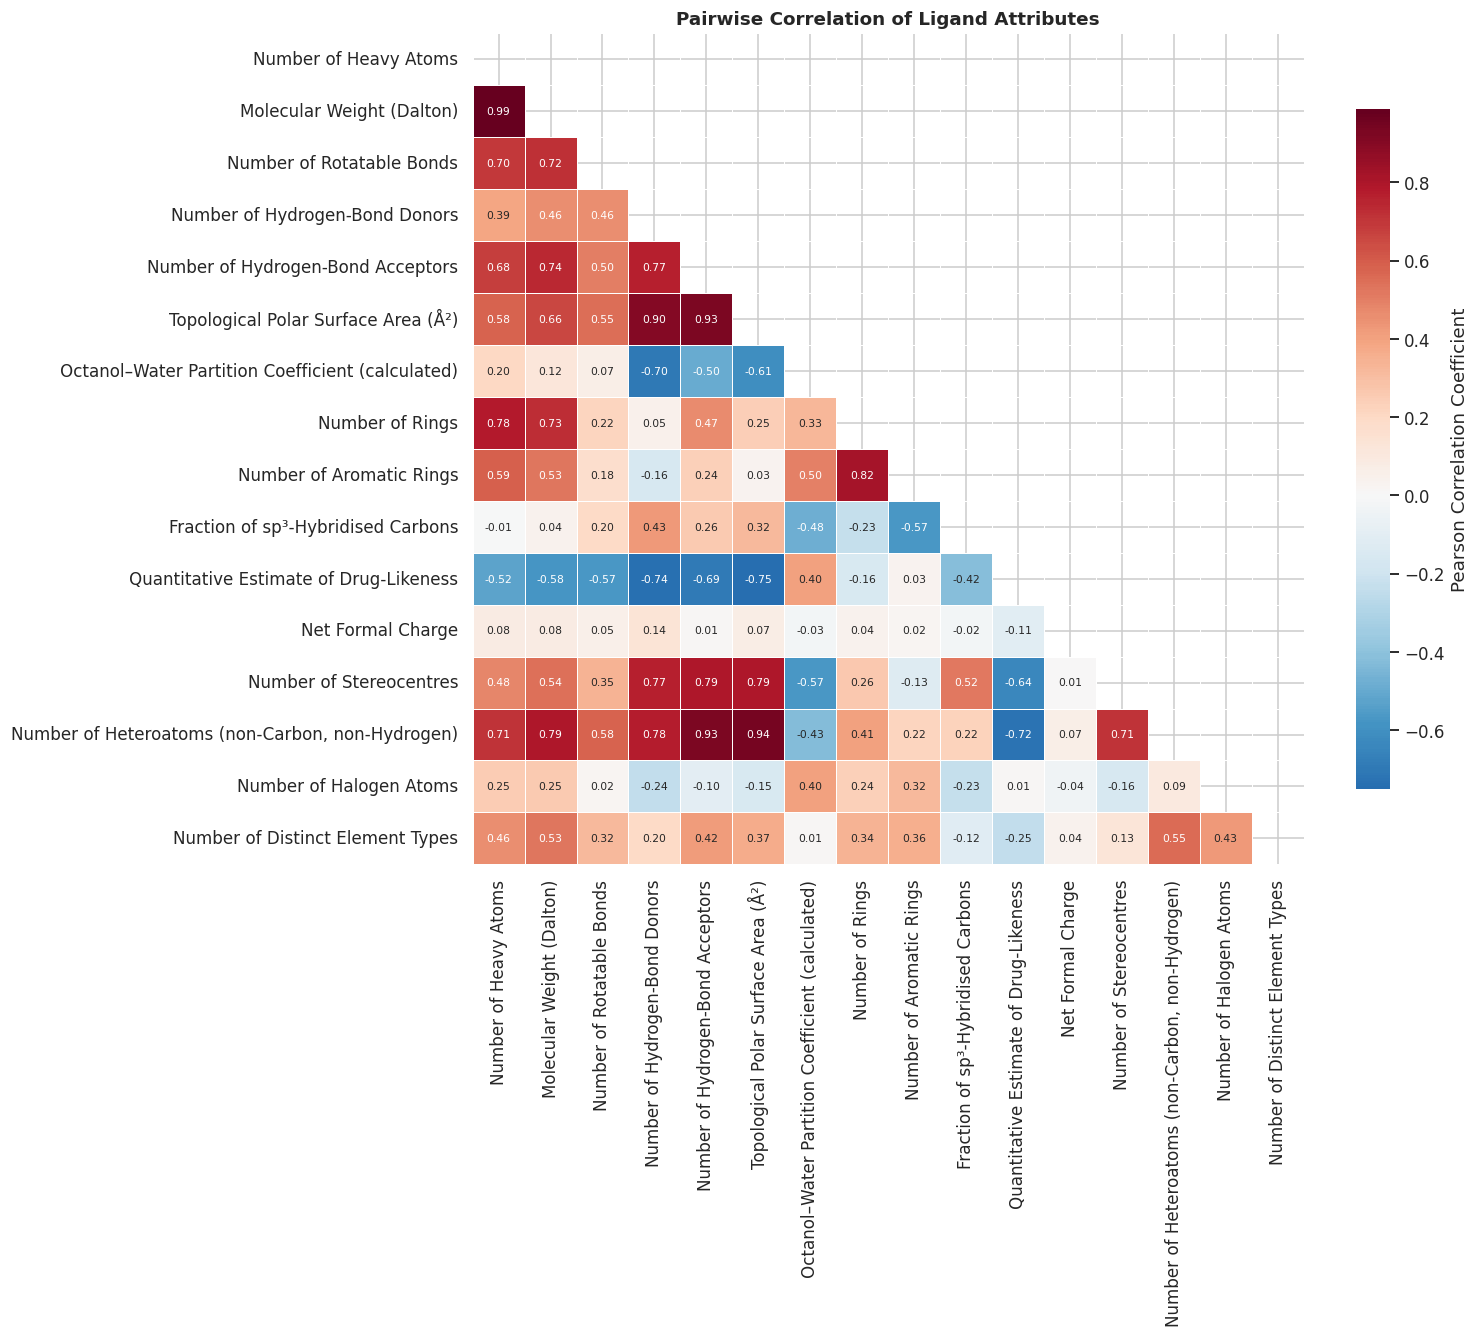
\includegraphics[width=\linewidth,height=0.78\textheight,keepaspectratio]{media/media/image36.png}
\caption{Pairwise Pearson correlation of the sixteen ligand descriptors}\label{fig:appendix-dataset-4}
\end{figure}

\begin{figure}[!htbp]
\centering

\includegraphics[width=\linewidth,height=0.78\textheight,keepaspectratio]{media/media/image37.png}
\caption{Two-dimensional attribute mappings with points coloured by QED. The JKU reference ligands are marked. R denotes the Pearson correlation}\label{fig:appendix-dataset-5}
\end{figure}

\begin{figure}[!htbp]
\centering
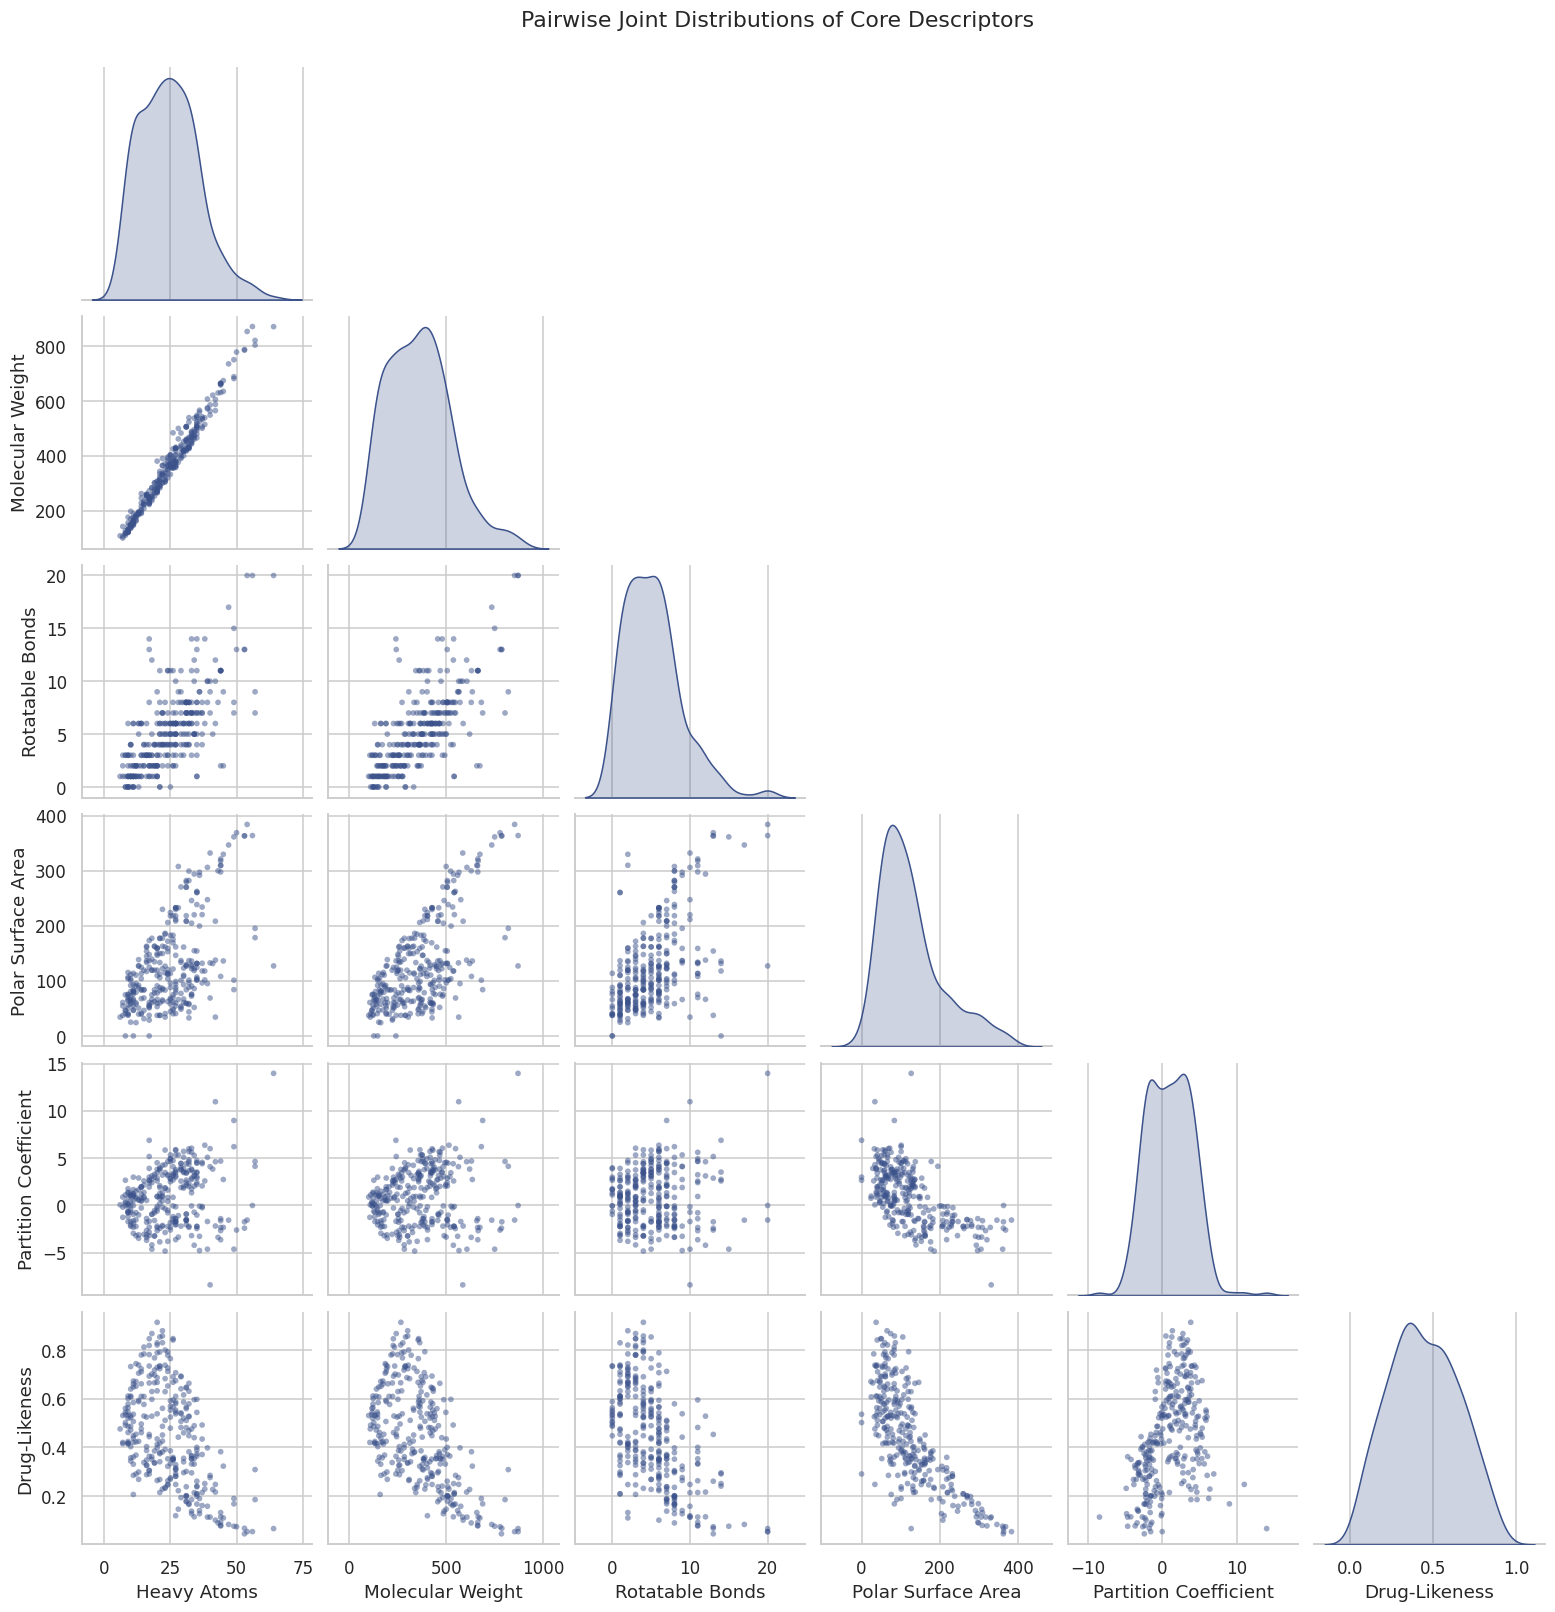
\includegraphics[width=\linewidth,height=0.78\textheight,keepaspectratio]{media/media/image38.png}
\caption{Pairwise joint distributions of six core descriptors with kernel-density estimates on the diagonal}\label{fig:appendix-dataset-6}
\end{figure}

\hypertarget{principal-component-analysis-chemical-space}{%
\section{Principal-Component Analysis --- Chemical Space}\label{principal-component-analysis-chemical-space}}

Summarising this correlated space, a principal-component analysis was run on the sixteen standardised ligand descriptors. Two components already capture roughly two-thirds of the variance (PC1 \ensuremath{\approx} 45\%, PC2 \ensuremath{\approx} 23\%) and four reach about 81\% (Figure~\ref{fig:appendix-dataset-7}), showing that only a few underlying factors govern the set's diversity. The first component is a size-and-polarity axis. Heavy-atom count, molecular weight, hydrogen-bond acceptors and donors, polar surface area, heteroatom and stereocentre counts all load strongly and positively, while QED loads strongly negative, so moving along PC1 trades rising size, polarity and complexity against falling drug-likeness. The second component separates flat, lipophilic, aromatic, halogenated scaffolds (positive loadings on aromatic rings, cLogP, ring count and halogen count) from saturated, sp\textsuperscript{3}-rich, hydrogen-bond-donating ones. The minor components capture halogenation and element diversity (PC3) and net formal charge (PC4). Overlaying the per-ligand difficulty of reproducing the crystal pose on the score plot, it rises towards positive PC1 (Figure~\ref{fig:appendix-dataset-8}), identifying molecular size and flexibility, not aromatic or lipophilic character, as the dominant driver of docking difficulty.

\begin{figure}[!htbp]
\centering
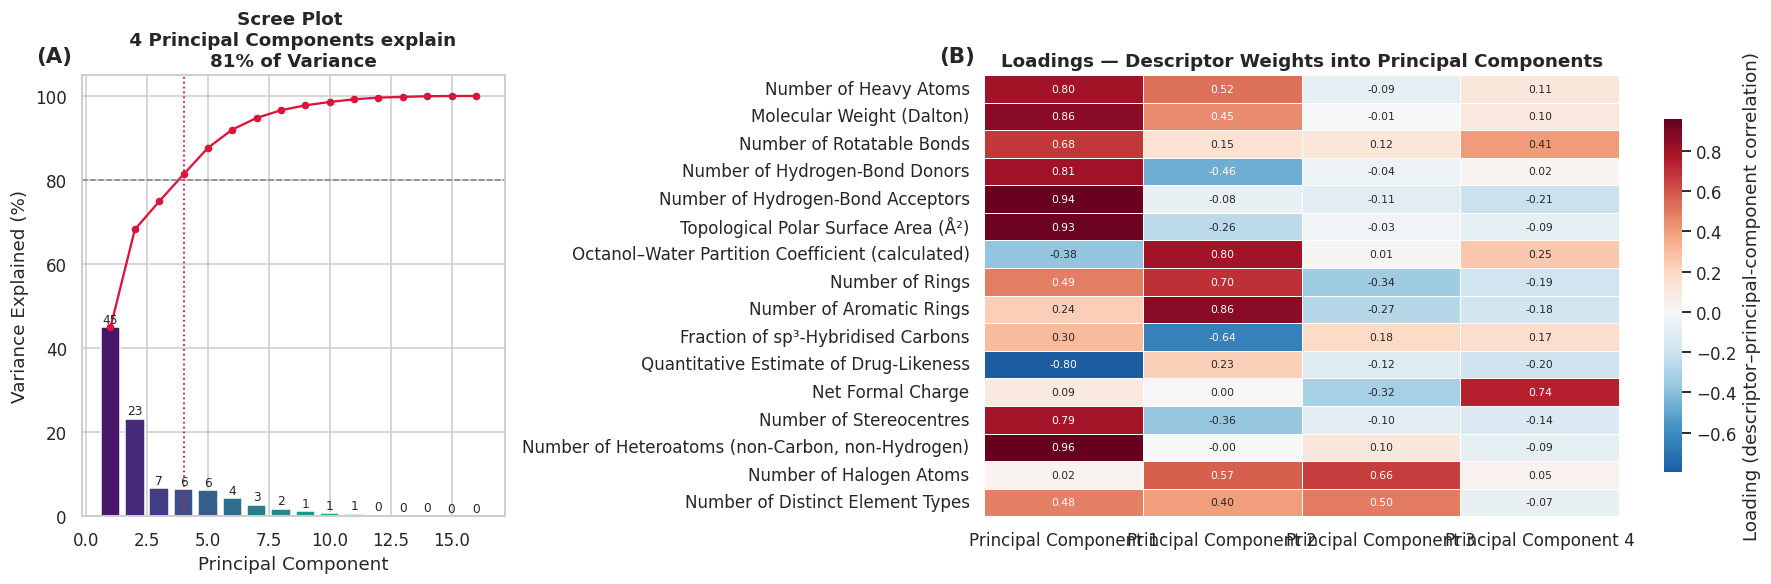
\includegraphics[width=\linewidth,height=0.78\textheight,keepaspectratio]{media/media/image39.png}
\caption{Principal-component analysis of the standardised ligand descriptors. Scree plot of explained variance (left) and component loadings (right)}\label{fig:appendix-dataset-7}
\end{figure}

\begin{figure}[!htbp]
\centering

\includegraphics[width=\linewidth,height=0.78\textheight,keepaspectratio]{media/media/image40.png}
\caption{PCA biplot with descriptor loadings (left) and PC scores coloured by conformer-generation difficulty (right). The experimentally validated ligands are projected into the same space}\label{fig:appendix-dataset-8}
\end{figure}

\hypertarget{receptor-profile}{%
\section{Receptor Profile}\label{receptor-profile}}

The receptor side is equally varied (Figure~\ref{fig:appendix-dataset-9}). A typical complex resolves 472 residues (interquartile range 306 to 778) and is a monomer or dimer, but the distribution has a long tail of large multi-chain assemblies running to forty chains and several thousand residues. Critically, 89\% of the complexes keep at least one cofactor or hetero-component, so the binding environments are realistic rather than artificially stripped. Ligand size is essentially independent of receptor size, meaning small ligands are docked into both small and very large pockets and receptor dimensions cannot act as a confounding shortcut.

\begin{figure}[!htbp]
\centering

\includegraphics[width=\linewidth,height=0.78\textheight,keepaspectratio]{media/media/image41.png}
\caption{Receptor profile. Resolved residues, chains per complex, distinct cofactor types and ligand-versus-receptor size}\label{fig:appendix-dataset-9}
\end{figure}

\hypertarget{conformer-generation-difficulty}{%
\section{Conformer-Generation Difficulty}\label{conformer-generation-difficulty}}

The single ETKDGv3+UFF starting conformer supplied with each ligand gives a lower-bound estimate of how far a docking engine must move the ligand to recover the crystal pose. The symmetry-corrected RMSD between this start conformer and the crystallographic pose has a median of 1.56\angstrom{}, and only 65\% of conformers fall within 2\angstrom{} of the answer (Figure~\ref{fig:appendix-dataset-10}). This deviation grows steadily with rotatable-bond count (r = +0.75) and heavy-atom count (r = +0.80), quantifying the search burden the set imposes and confirming that ligand size and flexibility are its principal sources of difficulty.

\begin{figure}[!htbp]
\centering

\includegraphics[width=\linewidth,height=0.78\textheight,keepaspectratio]{media/media/image42.png}
\caption{Conformer-generation difficulty. The start-conformer-to-crystal RMSD distribution (left) and its dependence on rotatable bonds (centre) and heavy-atom count (right)}\label{fig:appendix-dataset-10}
\end{figure}

\hypertarget{contrast-with-the-functionally-tested-ligands}{%
\section{Contrast with the Functionally Tested Ligands}\label{contrast-with-the-functionally-tested-ligands}}

The geometry-optimised Orai1 ligands were characterised with the identical descriptor pipeline and projected onto the same chemical-space maps for comparison. Unlike the benchmark complexes, these compounds are experimental and carry no crystallographic reference pose, so their binding modes must be predicted. Their physicochemical profile is markedly narrower and more lead-like than the benchmark set (Table~\ref{tab:appendix-orai-descriptors}). With molecular weights of 225 to 396 Da, at most 28 heavy atoms, four to seven rotatable bonds, a single hydrogen-bond donor and polar surface areas below 65\angstrom{}\textsuperscript{2}, all three pass Lipinski's rule of five with zero violations and show QED values of roughly 0.75 to 0.81 (above the benchmark median of 0.44). Across the distribution figures the reference ligands consistently land on the small, drug-like, aromatic-lipophilic side of every attribute, and in the principal-component projection they cluster at negative PC1 and positive PC2, the compact, lead-like, comparatively easy-to-reproduce corner of the benchmark's chemical space.

\begin{longtable}[]{@{}
  >{\raggedright\arraybackslash}p{(\columnwidth - 14\tabcolsep) * \real{0.2278}}
  >{\raggedright\arraybackslash}p{(\columnwidth - 14\tabcolsep) * \real{0.1103}}
  >{\raggedright\arraybackslash}p{(\columnwidth - 14\tabcolsep) * \real{0.1103}}
  >{\raggedright\arraybackslash}p{(\columnwidth - 14\tabcolsep) * \real{0.1030}}
  >{\raggedright\arraybackslash}p{(\columnwidth - 14\tabcolsep) * \real{0.1397}}
  >{\raggedright\arraybackslash}p{(\columnwidth - 14\tabcolsep) * \real{0.1175}}
  >{\raggedright\arraybackslash}p{(\columnwidth - 14\tabcolsep) * \real{0.0956}}
  >{\raggedright\arraybackslash}p{(\columnwidth - 14\tabcolsep) * \real{0.0957}}@{}}
\caption[Orai1 Ligand Physicochemical Descriptors]{Physicochemical Descriptors of the Geometry-Optimised Orai1 Reference Ligands}\tabularnewline
\toprule\noalign{}
{\raggedright \textbf{Ligand}} & {\raggedright \textbf{MW (Da)}} & \shortstack[l]{\textbf{Heavy}\\\textbf{atoms}\strut} & \shortstack[l]{\textbf{Rot.}\\\textbf{bonds}\strut} & {\raggedright \textbf{HBD / HBA}} & {\raggedright \textbf{TPSA (\angstrom{}\textsuperscript{2})}} & {\raggedright \textbf{cLogP}} & \shortstack[l]{\textbf{Ro5}\\\textbf{viol.}\strut} \\
\midrule\noalign{}
\endfirsthead
\caption[]{Physicochemical Descriptors of the Geometry-Optimised Orai1 Reference Ligands (continued)}\tabularnewline
\toprule\noalign{}
{\raggedright \textbf{Ligand}} & {\raggedright \textbf{MW (Da)}} & \shortstack[l]{\textbf{Heavy}\\\textbf{atoms}\strut} & \shortstack[l]{\textbf{Rot.}\\\textbf{bonds}\strut} & {\raggedright \textbf{HBD / HBA}} & {\raggedright \textbf{TPSA (\angstrom{}\textsuperscript{2})}} & {\raggedright \textbf{cLogP}} & \shortstack[l]{\textbf{Ro5}\\\textbf{viol.}\strut} \\
\midrule\noalign{}
\endhead
\bottomrule\noalign{}
\endlastfoot
2abp-NH2 & 225 & 17 & 6 & 1 / 2 & 35.3 & 0.77 & 0 \\
Synta-66 & 352 & 26 & 7 & 1 / 4 & 60.5 & 4.16 & 0 \\
GSK-7975A (deprot) & 396 & 28 & 4 & 1 / 4 & 64.0 & 3.62 & 0 \\
\end{longtable}
% RESOLVED 2026-07-26: Table 3 (main text) descriptors regenerated from the exact docked SDFs (Data/Ligands/JKU/pdbqt/*.sdf) via RDKit and now match this Appendix table: 2abp-NH2/2-APB C14H16BNO 225.1 Da/17/6; Synta-66 C20H17FN2O3 (no S) 352.4 Da/26/7; GSK-7975A deprot C18H11F5N3O2 396.3 Da/28/4. Identity note: docked 2abp-NH2 InChIKey BLZVCIGGICSWIG-UHFFFAOYSA-N == native 2-APB (neutral form), PubChem CID 1598 -- it is the same molecule, not a distinct analogue.
\labelcurrenttable{tab:appendix-orai-descriptors}

\hypertarget{suitability-of-the-dataset}{%
\section{Suitability of the Dataset}\label{suitability-of-the-dataset}}

This contrast is what makes the PoseBusters subset a sound calibration anchor. The benchmark brackets and clearly exceeds the chemical and structural complexity of the experimental Orai1 ligands. It is larger, more polar, more flexible and more diverse, and it sets a harder conformer-search problem. Reproducing the published performance of AutoDock Vina, DiffDock and EquiBind across this demanding, experimentally grounded set therefore shows the docking-and-validation pipeline working well within its tested range before it is applied to the smaller, lead-like JKU compounds. Testing the three tools across far more chemical diversity than the experimental targets demand, and grounding that test in experimentally resolved poses, supplies the objective reference that the experimental dataset itself cannot.

\hypertarget{ranking-recovery-statistics}{%
\chapter{Ranking-Recovery Statistics}\label{ranking-recovery-statistics}}

The following tables give the full statistics at each ranking depth for the top-k cumulative recovery of each variant. Recovery is reported for k = 1, 5, 10 and 15 over the N = 303 calibration complexes. Percentages are complex-level recovery rates and bracketed intervals are Wilson 95\% confidence intervals. Paired comparisons use McNemar\textquotesingle s exact test with Holm correction across the full 24-test family, where significance is marked as * p \textless{} 0.05, ** p \textless{} 0.01 and *** p \textless{} 0.001, and ns denotes not significant.

\begin{landscape}
\scriptsize
\setlength{\tabcolsep}{2pt}
\begin{longtable}[]{@{}
  >{\raggedright\arraybackslash}p{(\columnwidth - 6\tabcolsep) * \real{0.2500}}
  >{\raggedright\arraybackslash}p{(\columnwidth - 6\tabcolsep) * \real{0.2500}}
  >{\raggedright\arraybackslash}p{(\columnwidth - 6\tabcolsep) * \real{0.2500}}
  >{\raggedright\arraybackslash}p{(\columnwidth - 6\tabcolsep) * \real{0.2500}}@{}}
\caption{Top-k Recovery with Wilson 95\% Confidence Intervals}\tabularnewline
\toprule\noalign{}
{\raggedright \textbf{Variant}} & {\raggedright \textbf{k}} & {\raggedright \textbf{Near-native\% {[}95\% CI{]}}} & {\raggedright \textbf{Validity-aware\% {[}95\% CI{]}}} \\
\midrule\noalign{}
\endfirsthead
\caption[]{Top-k Recovery with Wilson 95\% Confidence Intervals (continued)}\tabularnewline
\toprule\noalign{}
{\raggedright \textbf{Variant}} & {\raggedright \textbf{k}} & {\raggedright \textbf{Near-native\% {[}95\% CI{]}}} & {\raggedright \textbf{Validity-aware\% {[}95\% CI{]}}} \\
\midrule\noalign{}
\endhead
\bottomrule\noalign{}
\endlastfoot
AutoDock Vina & 1 & 57.8 {[}52.1, 63.2{]} & 55.5 {[}49.8, 60.9{]} \\
& 5 & 79.2 {[}74.3, 83.4{]} & 77.9 {[}72.9, 82.2{]} \\
& 10 & 85.1 {[}80.7, 88.7{]} & 83.8 {[}79.3, 87.5{]} \\
& 15 & 87.5 {[}83.3, 90.7{]} & 86.1 {[}81.8, 89.6{]} \\
DiffDock (raw) & 1 & 33.7 {[}28.6, 39.2{]} & 17.8 {[}13.9, 22.5{]} \\
& 5 & 44.6 {[}39.1, 50.2{]} & 25.1 {[}20.5, 30.3{]} \\
& 10 & 48.2 {[}42.6, 53.8{]} & 28.4 {[}23.6, 33.7{]} \\
& 15 & 49.8 {[}44.2, 55.4{]} & 30.7 {[}25.8, 36.1{]} \\
DiffDock (gnina-opt) & 1 & 35.6 {[}30.5, 41.2{]} & 32.3 {[}27.3, 37.8{]} \\
& 5 & 49.2 {[}43.6, 54.8{]} & 46.2 {[}40.7, 51.8{]} \\
& 10 & 52.8 {[}47.2, 58.4{]} & 48.8 {[}43.3, 54.5{]} \\
& 15 & 56.1 {[}50.5, 61.6{]} & 51.5 {[}45.9, 57.1{]} \\
EquiBind (raw) & 1 & 1.3 {[}0.5, 3.3{]} & 0.7 {[}0.2, 2.4{]} \\
& 5 & 3.0 {[}1.6, 5.5{]} & 0.7 {[}0.2, 2.4{]} \\
& 10 & 4.0 {[}2.3, 6.8{]} & 0.7 {[}0.2, 2.4{]} \\
& 15 & 5.9 {[}3.8, 9.2{]} & 0.7 {[}0.2, 2.4{]} \\
EquiBind (gnina-opt) & 1 & 15.5 {[}11.9, 20.0{]} & 15.2 {[}11.6, 19.7{]} \\
& 5 & 19.8 {[}15.7, 24.7{]} & 19.1 {[}15.1, 23.9{]} \\
& 10 & 20.8 {[}16.6, 25.7{]} & 20.1 {[}16.0, 25.0{]} \\
& 15 & 21.1 {[}16.9, 26.1{]} & 20.5 {[}16.3, 25.4{]} \\
\end{longtable}
\labelcurrenttable{tab:appendix-top-k-recovery}
\end{landscape}

\begin{landscape}
\scriptsize
\setlength{\tabcolsep}{2pt}
\begin{longtable}[]{@{}
  >{\raggedright\arraybackslash}p{(\columnwidth - 12\tabcolsep) * \real{0.1429}}
  >{\raggedright\arraybackslash}p{(\columnwidth - 12\tabcolsep) * \real{0.1429}}
  >{\raggedright\arraybackslash}p{(\columnwidth - 12\tabcolsep) * \real{0.1429}}
  >{\raggedright\arraybackslash}p{(\columnwidth - 12\tabcolsep) * \real{0.1429}}
  >{\raggedright\arraybackslash}p{(\columnwidth - 12\tabcolsep) * \real{0.1429}}
  >{\raggedright\arraybackslash}p{(\columnwidth - 12\tabcolsep) * \real{0.1429}}
  >{\raggedright\arraybackslash}p{(\columnwidth - 12\tabcolsep) * \real{0.1429}}@{}}
\caption{Raw-to-gnina Refinement Effect on Cumulative Top-k Near-Native Recovery}\tabularnewline
\toprule\noalign{}
{\raggedright \textbf{Tool}} & {\raggedright \textbf{k}} & {\raggedright \textbf{raw\% \ensuremath{\rightarrow} gnina-opt\%}} & {\raggedright \textbf{discordant (raw-only / opt-only)}} & {\raggedright \textbf{p (raw)}} & {\raggedright \textbf{p (Holm)}} & {\raggedright \textbf{sig}} \\
\midrule\noalign{}
\endfirsthead
\caption[]{Raw-to-gnina Refinement Effect on Cumulative Top-k Near-Native Recovery (continued)}\tabularnewline
\toprule\noalign{}
{\raggedright \textbf{Tool}} & {\raggedright \textbf{k}} & {\raggedright \textbf{raw\% \ensuremath{\rightarrow} gnina-opt\%}} & {\raggedright \textbf{discordant (raw-only / opt-only)}} & {\raggedright \textbf{p (raw)}} & {\raggedright \textbf{p (Holm)}} & {\raggedright \textbf{sig}} \\
\midrule\noalign{}
\endhead
\bottomrule\noalign{}
\endlastfoot
DiffDock & 1 & 33.7 \ensuremath{\rightarrow} 35.6 & 2 / 8 & 0.109 & 0.109 & ns \\
& 5 & 44.6 \ensuremath{\rightarrow} 49.2 & 5 / 19 & 0.007 & 0.020 & * \\
& 10 & 48.2 \ensuremath{\rightarrow} 52.8 & 6 / 20 & 0.009 & 0.020 & * \\
& 15 & 49.8 \ensuremath{\rightarrow} 56.1 & 6 / 25 & 0.00088 & 0.004 & ** \\
EquiBind & 1 & 1.3 \ensuremath{\rightarrow} 15.5 & 1 / 44 & \textless1e-4 & \textless1e-4 & *** \\
& 5 & 3.0 \ensuremath{\rightarrow} 19.8 & 1 / 52 & \textless1e-4 & \textless1e-4 & *** \\
& 10 & 4.0 \ensuremath{\rightarrow} 20.8 & 1 / 52 & \textless1e-4 & \textless1e-4 & *** \\
& 15 & 5.9 \ensuremath{\rightarrow} 21.1 & 1 / 47 & \textless1e-4 & \textless1e-4 & *** \\
\multicolumn{7}{@{}p{\dimexpr\columnwidth-12\tabcolsep\relax}@{}}{\footnotesize%
Recovery here is the cumulative best-of-top-\emph{k} complex rate, in which a complex counts when \emph{any} of its top-\emph{k} poses is near-native. For DiffDock the top-\emph{k} pool is the same set of confidence-ranked poses before and after refinement, so its raw\,\ensuremath{\rightarrow}\,gnina gain is geometry repair alone, accumulated across ranks by the best-of-top-\emph{k} union rather than produced by any re-ordering. EquiBind has no native ranking, so its gnina variant is additionally re-ranked by gnina affinity, and its gain also reflects which pooled pose is drawn into the top \emph{k}. Both gains are therefore larger than the fixed-rank, per-pose near-native rate change of 0.1--0.7 (DiffDock) and 2.5--3.1 (EquiBind) percentage points reported in the Discussion, which holds each pose at its own rank and measures only the geometry repair of that same pose. Those per-rank changes are broken out by rank band in Table~\ref{tab:appendix-refinement-bands}.} \\
\end{longtable}
\labelcurrenttable{tab:appendix-refinement-mcnemar}
\end{landscape}

\begin{landscape}
\scriptsize
\setlength{\tabcolsep}{2pt}
\begin{longtable}[]{@{}
  >{\raggedright\arraybackslash}p{(\columnwidth - 14\tabcolsep) * \real{0.1400}}
  >{\raggedright\arraybackslash}p{(\columnwidth - 14\tabcolsep) * \real{0.2200}}
  >{\raggedright\arraybackslash}p{(\columnwidth - 14\tabcolsep) * \real{0.1067}}
  >{\raggedright\arraybackslash}p{(\columnwidth - 14\tabcolsep) * \real{0.1067}}
  >{\raggedright\arraybackslash}p{(\columnwidth - 14\tabcolsep) * \real{0.1067}}
  >{\raggedright\arraybackslash}p{(\columnwidth - 14\tabcolsep) * \real{0.1067}}
  >{\raggedright\arraybackslash}p{(\columnwidth - 14\tabcolsep) * \real{0.1066}}
  >{\raggedright\arraybackslash}p{(\columnwidth - 14\tabcolsep) * \real{0.1066}}@{}}
\caption{Fixed-Rank Refinement Gain in Near-Native and Validity Rates by Pose-Rank Band}\tabularnewline
\toprule\noalign{}
{\raggedright \textbf{Tool}} & {\raggedright \textbf{Criterion}} & {\raggedright \textbf{1--10 smina}} & {\raggedright \textbf{1--10 gnina}} & {\raggedright \textbf{11--20 smina}} & {\raggedright \textbf{11--20 gnina}} & {\raggedright \textbf{21--30 smina}} & {\raggedright \textbf{21--30 gnina}} \\
\midrule\noalign{}
\endfirsthead
\caption[]{Fixed-Rank Refinement Gain in Near-Native and Validity Rates by Pose-Rank Band (continued)}\tabularnewline
\toprule\noalign{}
{\raggedright \textbf{Tool}} & {\raggedright \textbf{Criterion}} & {\raggedright \textbf{1--10 smina}} & {\raggedright \textbf{1--10 gnina}} & {\raggedright \textbf{11--20 smina}} & {\raggedright \textbf{11--20 gnina}} & {\raggedright \textbf{21--30 smina}} & {\raggedright \textbf{21--30 gnina}} \\
\midrule\noalign{}
\endhead
\bottomrule\noalign{}
\endlastfoot
DiffDock & near-native & +0.6 & +0.7 & +0.1 & +0.1 & +0.5 & +0.4 \\
DiffDock & PoseBusters-valid & +51 & +52 & +55 & +57 & +59 & +63 \\
DiffDock & near-native + PB-valid & +12.4 & +12.1 & +7.3 & +7.2 & +4.7 & +4.8 \\
EquiBind & near-native & +2.6 & +3.1 & +2.5 & +2.8 & +2.6 & +3.0 \\
EquiBind & PoseBusters-valid & +37 & +48 & +36 & +50 & +37 & +51 \\
EquiBind & near-native + PB-valid & +2.5 & +3.0 & +2.7 & +3.2 & +2.8 & +3.2 \\
\multicolumn{8}{@{}p{\dimexpr\columnwidth-14\tabcolsep\relax}@{}}{\footnotesize%
Entries are the change in the per-rank rate (percentage points) averaged within each pose-rank band, with every pose held at its own confidence rank for DiffDock or generation rank for EquiBind, so no re-ranking is involved. The near-native gnina bands span 0.1 to 0.7 percentage points for DiffDock and 2.8 to 3.1 for EquiBind, and the smina bands span 0.1 to 0.6 and 2.5 to 2.6, which give the composite 0.1--0.7 and 2.5--3.1 ranges quoted in the Discussion and in the note to Table~\ref{tab:appendix-refinement-mcnemar}. The derived near-native + PB-valid column is shown for context and is near-nativeness and validity by construction.} \\
\end{longtable}
\labelcurrenttable{tab:appendix-refinement-bands}
\end{landscape}

\begin{landscape}
\scriptsize
\setlength{\tabcolsep}{2pt}
\begin{longtable}[]{@{}
  >{\raggedright\arraybackslash}p{(\columnwidth - 8\tabcolsep) * \real{0.2000}}
  >{\raggedright\arraybackslash}p{(\columnwidth - 8\tabcolsep) * \real{0.2000}}
  >{\raggedright\arraybackslash}p{(\columnwidth - 8\tabcolsep) * \real{0.2000}}
  >{\raggedright\arraybackslash}p{(\columnwidth - 8\tabcolsep) * \real{0.2001}}
  >{\raggedright\arraybackslash}p{(\columnwidth - 8\tabcolsep) * \real{0.2001}}@{}}
\caption{Cross-Tool Comparisons of Near-Native Recovery}\tabularnewline
\toprule\noalign{}
{\raggedright \textbf{Comparison (near-native\%)}} & {\raggedright \textbf{k = 1}} & {\raggedright \textbf{k = 5}} & {\raggedright \textbf{k = 10}} & {\raggedright \textbf{k = 15}} \\
\midrule\noalign{}
\endfirsthead
\caption[]{Cross-Tool Comparisons of Near-Native Recovery (continued)}\tabularnewline
\toprule\noalign{}
{\raggedright \textbf{Comparison (near-native\%)}} & {\raggedright \textbf{k = 1}} & {\raggedright \textbf{k = 5}} & {\raggedright \textbf{k = 10}} & {\raggedright \textbf{k = 15}} \\
\midrule\noalign{}
\endhead
\bottomrule\noalign{}
\endlastfoot
AutoDock vs DiffDock (raw) & 57.8 vs 33.7 & 79.2 vs 44.6 & 85.1 vs 48.2 & 87.5 vs 49.8 \\
AutoDock vs DiffDock (gnina-opt) & 57.8 vs 35.6 & 79.2 vs 49.2 & 85.1 vs 52.8 & 87.5 vs 56.1 \\
DiffDock (gnina-opt) vs EquiBind (gnina-opt) & 35.6 vs 15.5 & 49.2 vs 19.8 & 52.8 vs 20.8 & 56.1 vs 21.1 \\
AutoDock vs EquiBind (gnina-opt) & 57.8 vs 15.5 & 79.2 vs 19.8 & 85.1 vs 20.8 & 87.5 vs 21.1 \\
\end{longtable}
\labelcurrenttable{tab:appendix-cross-tool-mcnemar}
\end{landscape}

\begin{landscape}
\scriptsize
\setlength{\tabcolsep}{2pt}
\begin{longtable}[]{@{}
  >{\raggedright\arraybackslash}p{(\columnwidth - 8\tabcolsep) * \real{0.2000}}
  >{\raggedright\arraybackslash}p{(\columnwidth - 8\tabcolsep) * \real{0.2000}}
  >{\raggedright\arraybackslash}p{(\columnwidth - 8\tabcolsep) * \real{0.2000}}
  >{\raggedright\arraybackslash}p{(\columnwidth - 8\tabcolsep) * \real{0.2001}}
  >{\raggedright\arraybackslash}p{(\columnwidth - 8\tabcolsep) * \real{0.2001}}@{}}
\caption{Accurate-but-Invalid Share by Ranking Depth}\tabularnewline
\toprule\noalign{}
{\raggedright \textbf{Variant}} & {\raggedright \textbf{k = 1}} & {\raggedright \textbf{k = 5}} & {\raggedright \textbf{k = 10}} & {\raggedright \textbf{k = 15}} \\
\midrule\noalign{}
\endfirsthead
\caption[]{Accurate-but-Invalid Share by Ranking Depth (continued)}\tabularnewline
\toprule\noalign{}
{\raggedright \textbf{Variant}} & {\raggedright \textbf{k = 1}} & {\raggedright \textbf{k = 5}} & {\raggedright \textbf{k = 10}} & {\raggedright \textbf{k = 15}} \\
\midrule\noalign{}
\endhead
\bottomrule\noalign{}
\endlastfoot
AutoDock Vina & 2.3 {[}1.1, 4.7{]} & 1.3 & 1.3 & 1.3 \\
DiffDock (raw) & 15.8 {[}12.2, 20.4{]} & 19.5 & 19.8 & 19.1 \\
DiffDock (gnina-opt) & 3.3 & 3.0 & 4.0 & 4.6 \\
EquiBind (raw) & 0.7 & 2.3 & 3.3 & 5.3 \\
EquiBind (gnina-opt) & 0.3 & 0.7 & 0.7 & 0.7 \\
\end{longtable}
\labelcurrenttable{tab:appendix-accurate-invalid}
\end{landscape}
